\documentclass[a4paper]{article}

\usepackage[fontset=fandol]{ctex}
\usepackage{amsmath, amssymb}
\usepackage{graphicx}
\usepackage[margin=2.3cm]{geometry}
\usepackage[most]{tcolorbox}
\usepackage{listings}
\usepackage{hyperref}
\usepackage{booktabs}
\usepackage{float}
\usepackage{xcolor}

\lstset{
    language=Python,
    basicstyle=\ttfamily\small,
    keywordstyle=\color{blue},
    stringstyle=\color{red!60!black},
    commentstyle=\color{green!50!black},
    breaklines=true,
    frame=single,
    numbers=left,
    numberstyle=\tiny\color{gray}
}

\newtcolorbox{knowledgebox}[1]{
    enhanced,
    colback=blue!5!white,
    colframe=blue!70!black,
    colbacktitle=blue!70!black,
    coltitle=white,
    fonttitle=\bfseries,
    title=#1,
    sharp corners
}

\newtcolorbox{importantbox}[1]{
    enhanced,
    colback=yellow!10!white,
    colframe=yellow!70!black,
    colbacktitle=yellow!70!black,
    coltitle=black,
    fonttitle=\bfseries,
    title=#1,
    sharp corners
}

\newtcolorbox{warningbox}[1]{
    enhanced,
    colback=red!5!white,
    colframe=red!70!black,
    colbacktitle=red!70!black,
    coltitle=white,
    fonttitle=\bfseries,
    title=#1,
    sharp corners
}

\begin{document}

\begin{titlepage}
\centering
{\Large 课程讲义\par}
\vspace{1.2cm}
{\huge\bfseries Language models for autoformalization and theorem proving\par}
\vspace{0.6cm}
{\Large CS294/194-280: Advanced Large Language Model Agents\par}
\vspace{0.4cm}
{\large Kaiyu Yang, Meta FAIR\par}
\vspace{0.4cm}
{\large 中文教材化讲义 / Codex Harness Build\par}
\vspace{0.8cm}
\includegraphics[width=0.84\textwidth,height=0.38\textheight,keepaspectratio]{cover.jpg}\par
\vfill
\begin{tcolorbox}[width=0.92\textwidth,colback=black!2!white,colframe=black!60,sharp corners]
\textbf{课程页}：\href{https://rdi.berkeley.edu/adv-llm-agents/sp25}{Berkeley RDI SP25 course page}\par
\textbf{录播}：\href{https://www.youtube.com/live/cLhWEyMQ4mQ}{YouTube recording}\par
\textbf{slides}：\href{https://rdi.berkeley.edu/adv-llm-agents/slides/mathverification.pdf}{mathverification.pdf}\par
\textbf{补充 readings}：LeanDojo / Autoformalization with LLMs / Autoformalizing Euclidean Geometry
\end{tcolorbox}
\end{titlepage}

\tableofcontents
\newpage

\section{本讲学习目标}

本讲的目标不是简单罗列 theorem proving 论文，而是把形式推理任务拆成一个清晰的概念地图。读完本讲后，读者应当能够回答：

\begin{itemize}
\item 为什么 current math LLM 的主流训练 recipe 还不足以解决 formal reasoning。
\item formal specification、verification、theorem proving、proof search、autoformalization 各自的输入输出是什么。
\item proof assistant 为什么是 advanced agents 的理想 environment 之一。
\item LeanDojo、ReProver、LIPS 分别在 theorem proving 栈中解决了什么 bottleneck。
\item 为什么 autoformalization 的真正难点在 reasoning gaps、semantic equivalence 和 diagrammatic reasoning。
\end{itemize}

\section{背景与问题设置}

\subsection{为什么“会做数学题”不等于“会 formal reasoning”}

Kaiyu Yang 在开头先回顾了 math/coding arms race，并指出当前 math LLM 的训练 recipe 非常清晰：强预训练模型 + 数学监督数据的 SFT + 在可验证任务上的 RL。其抽象形式可以写成
\[
\theta^{\star} = \operatorname{RL}\!\left(\operatorname{SFT}\!\left(\theta_{0}; \mathcal{D}_{\mathrm{math}}\right); \mathcal{R}_{\mathrm{verify}}\right).
\]
这里 $\theta_0$ 是 base model，$\mathcal{D}_{\mathrm{math}}$ 是数学数据，$\mathcal{R}_{\mathrm{verify}}$ 是 verification-derived reward。这个 recipe 在 AIME、competition math 或 coding 上很强，但它并不自动给出 formal reasoning 能力。

\begin{figure}[H]
\centering
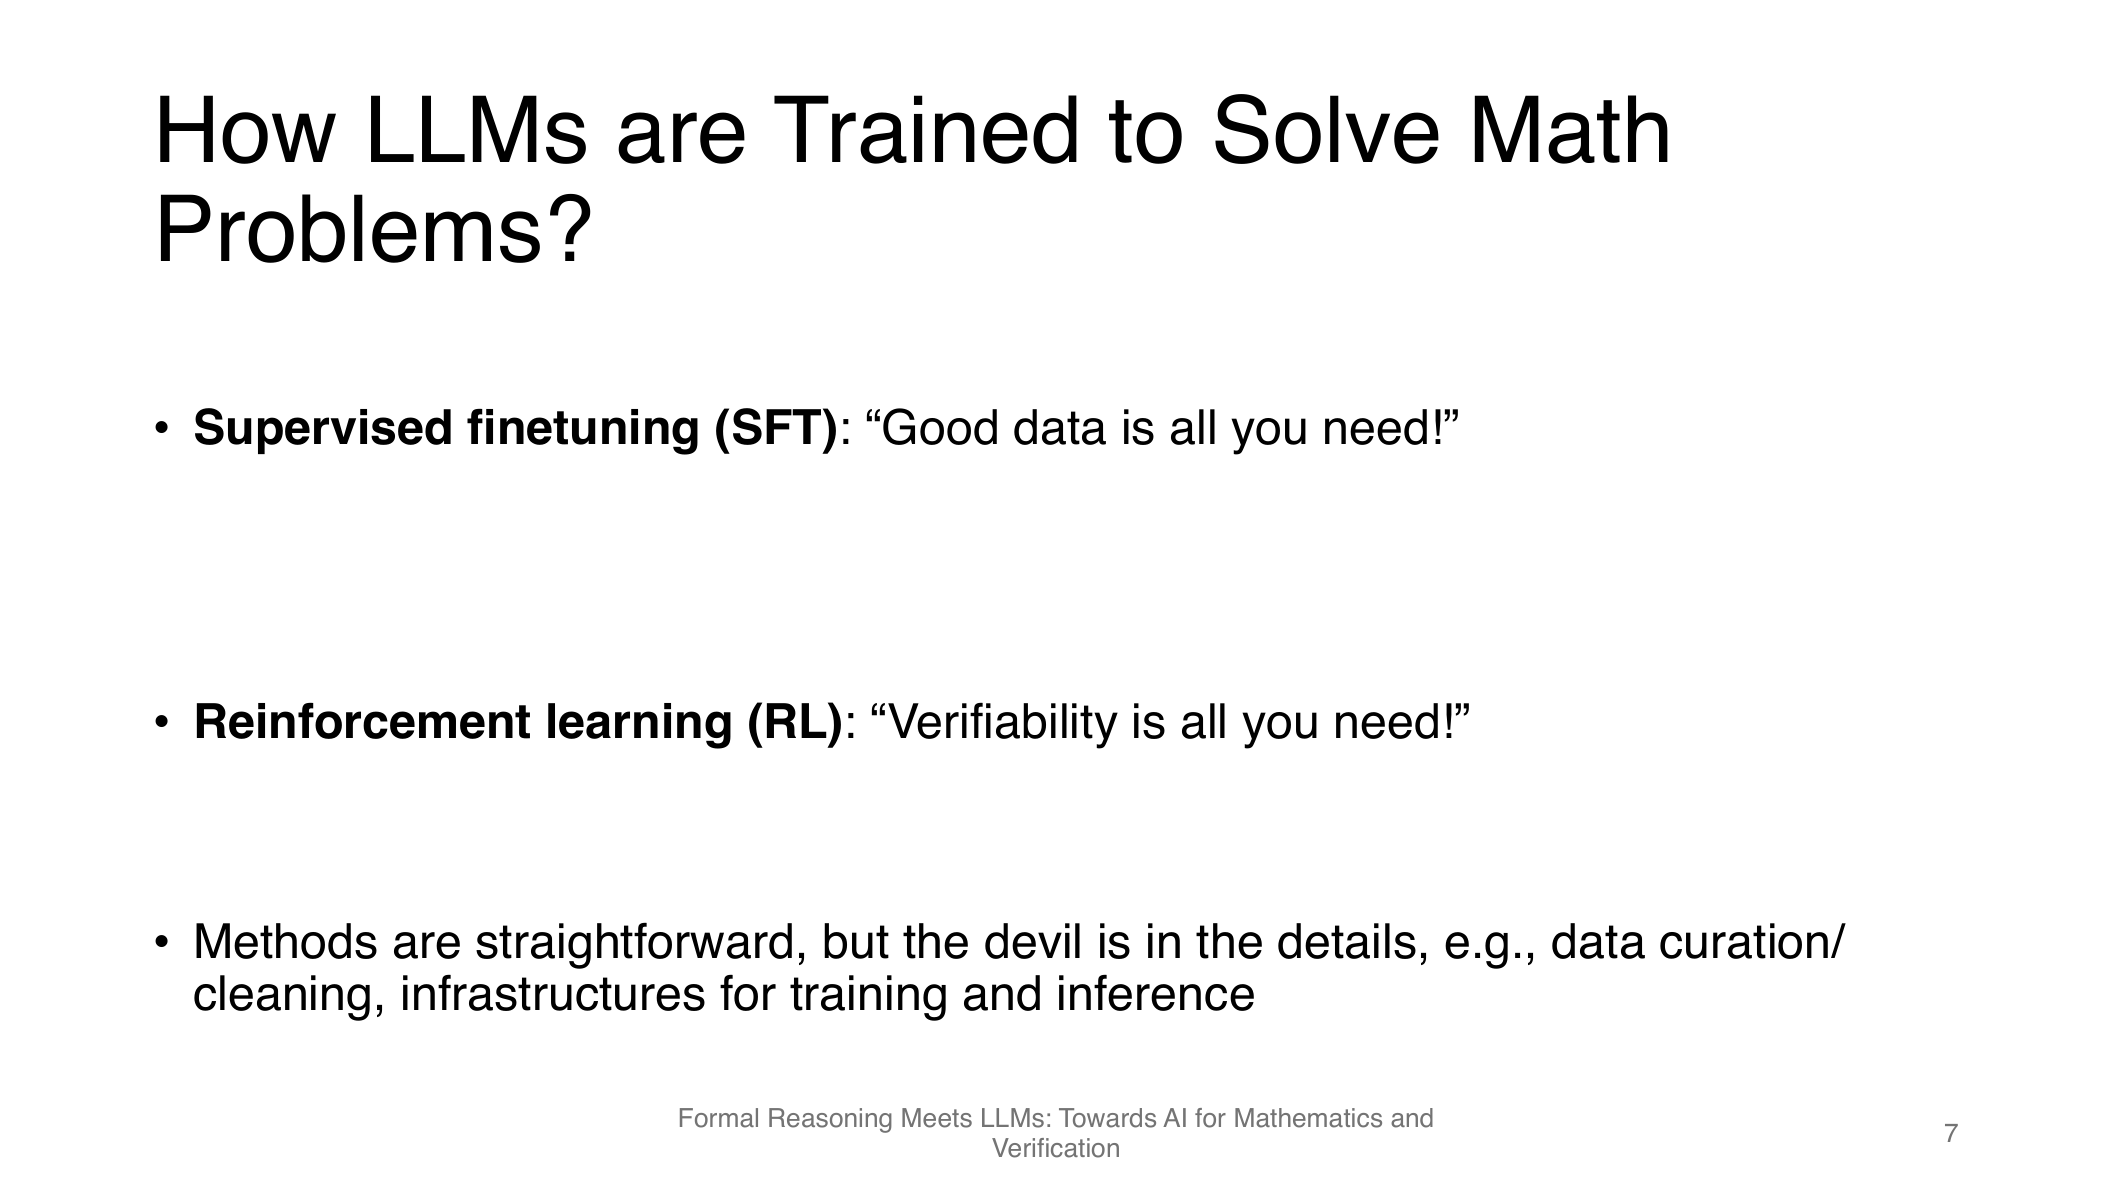
\includegraphics[width=0.82\textwidth]{figures/lec09_fig_001.png}
\caption{当前 math LLM 的主流训练 recipe。}
\end{figure}

问题在于：很多 benchmark 只要求猜对答案，却不要求写出 machine-checkable 的证明。于是模型也许能在\textbf{answer guessing}上表现很好，但仍然不会处理 formal theorem statement、proof states、premise retrieval 或 semantic equivalence。

\subsection{两个 gap：advanced math 与 valid proofs}

Slides 很明确地给出两个 gap。第一，\textbf{Pre-college Math $\rightarrow$ Advanced Math}：现有成功大多发生在竞赛或中学以上但仍然高度结构化的问题上。第二，\textbf{Guessing Answers $\rightarrow$ Writing Proofs}：从选一个对答案，到构造一条 checker 接受的 formal proof，是质变而不是量变。

\begin{figure}[H]
\centering
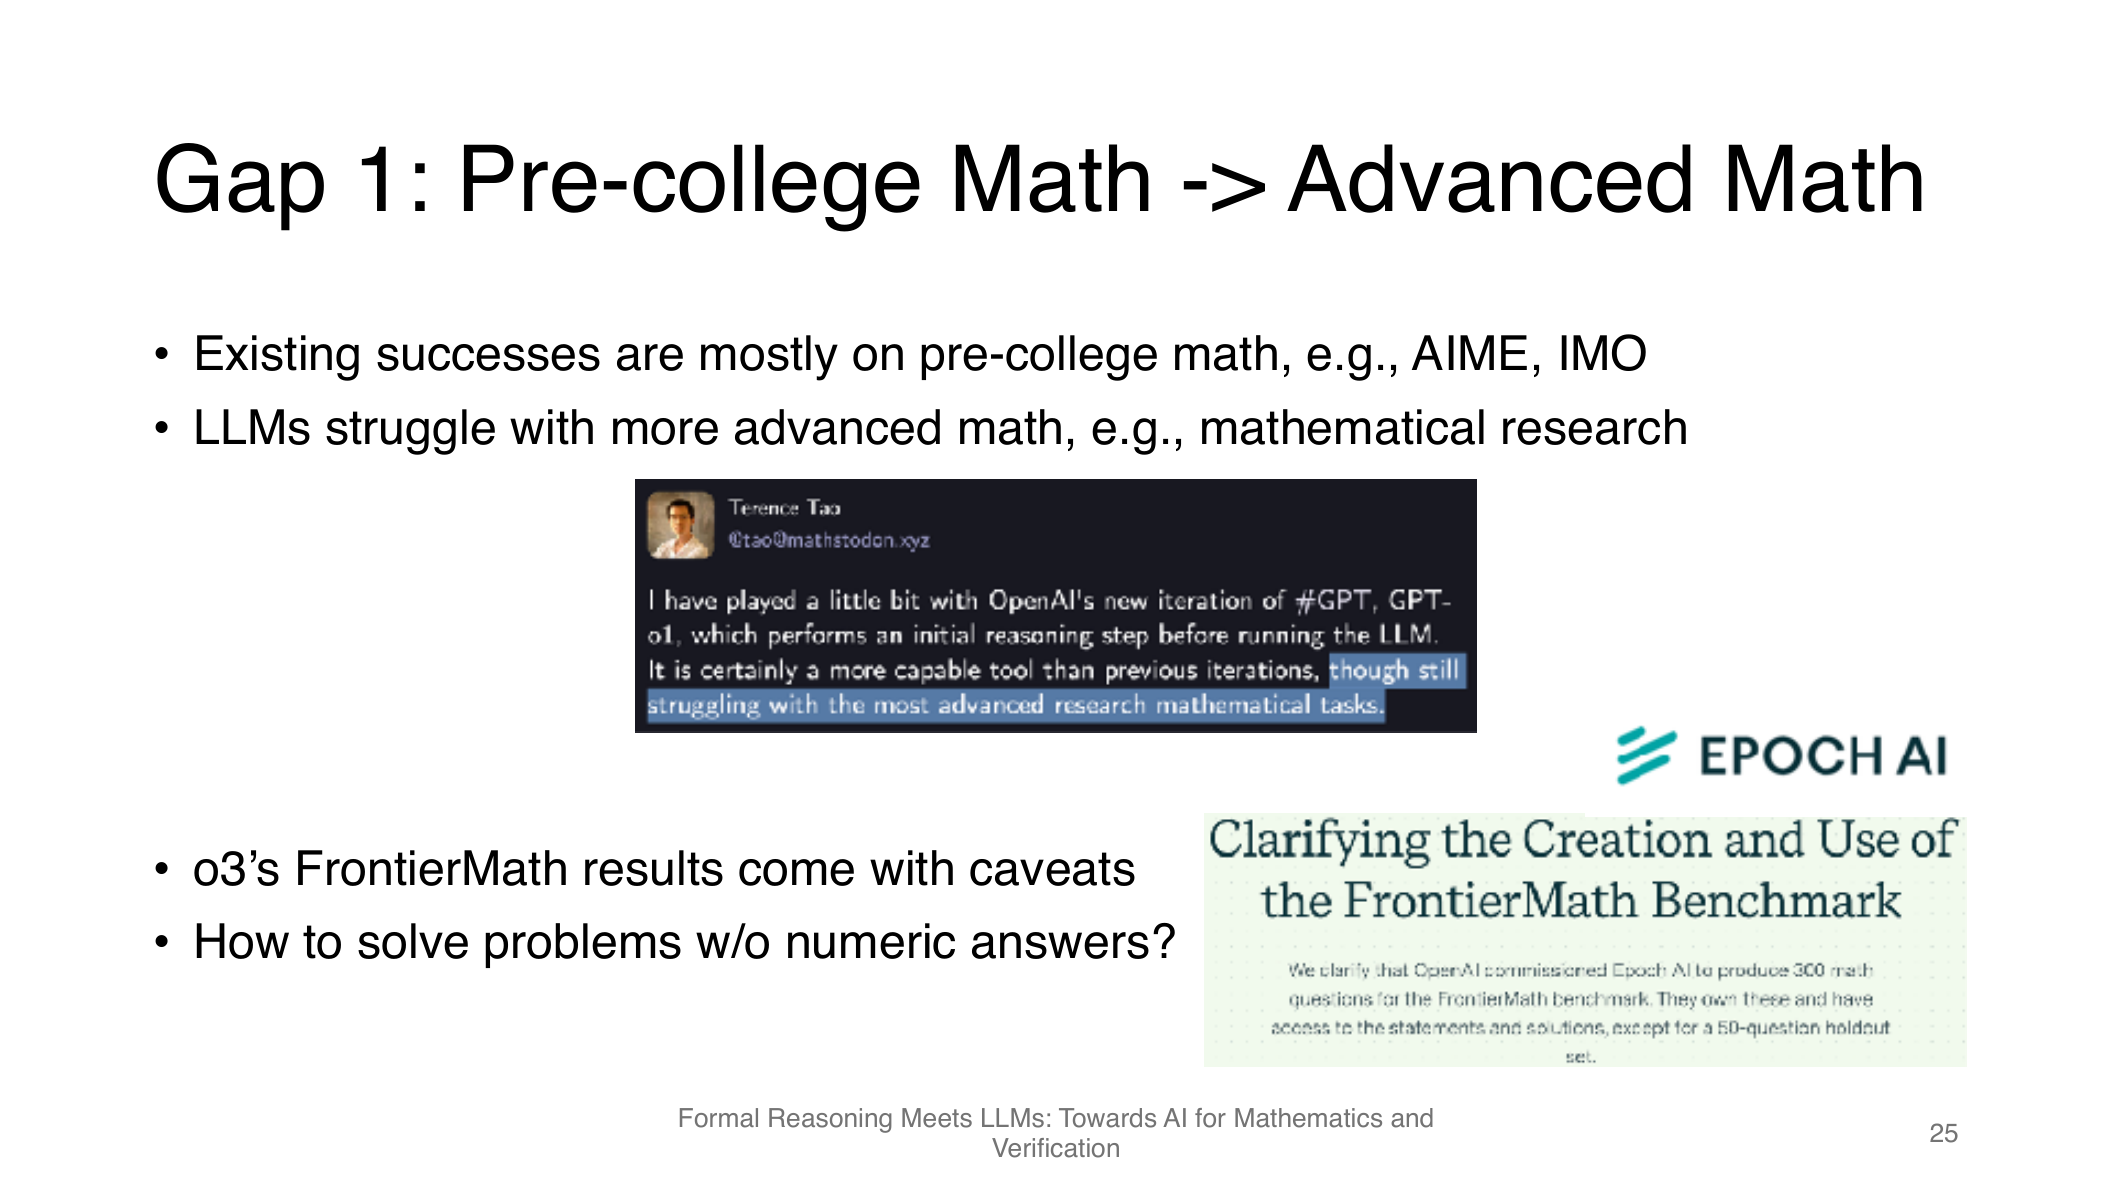
\includegraphics[width=0.80\textwidth]{figures/lec09_fig_002.png}
\caption{从 pre-college math 到 advanced math 的能力 gap。}
\end{figure}

\begin{figure}[H]
\centering
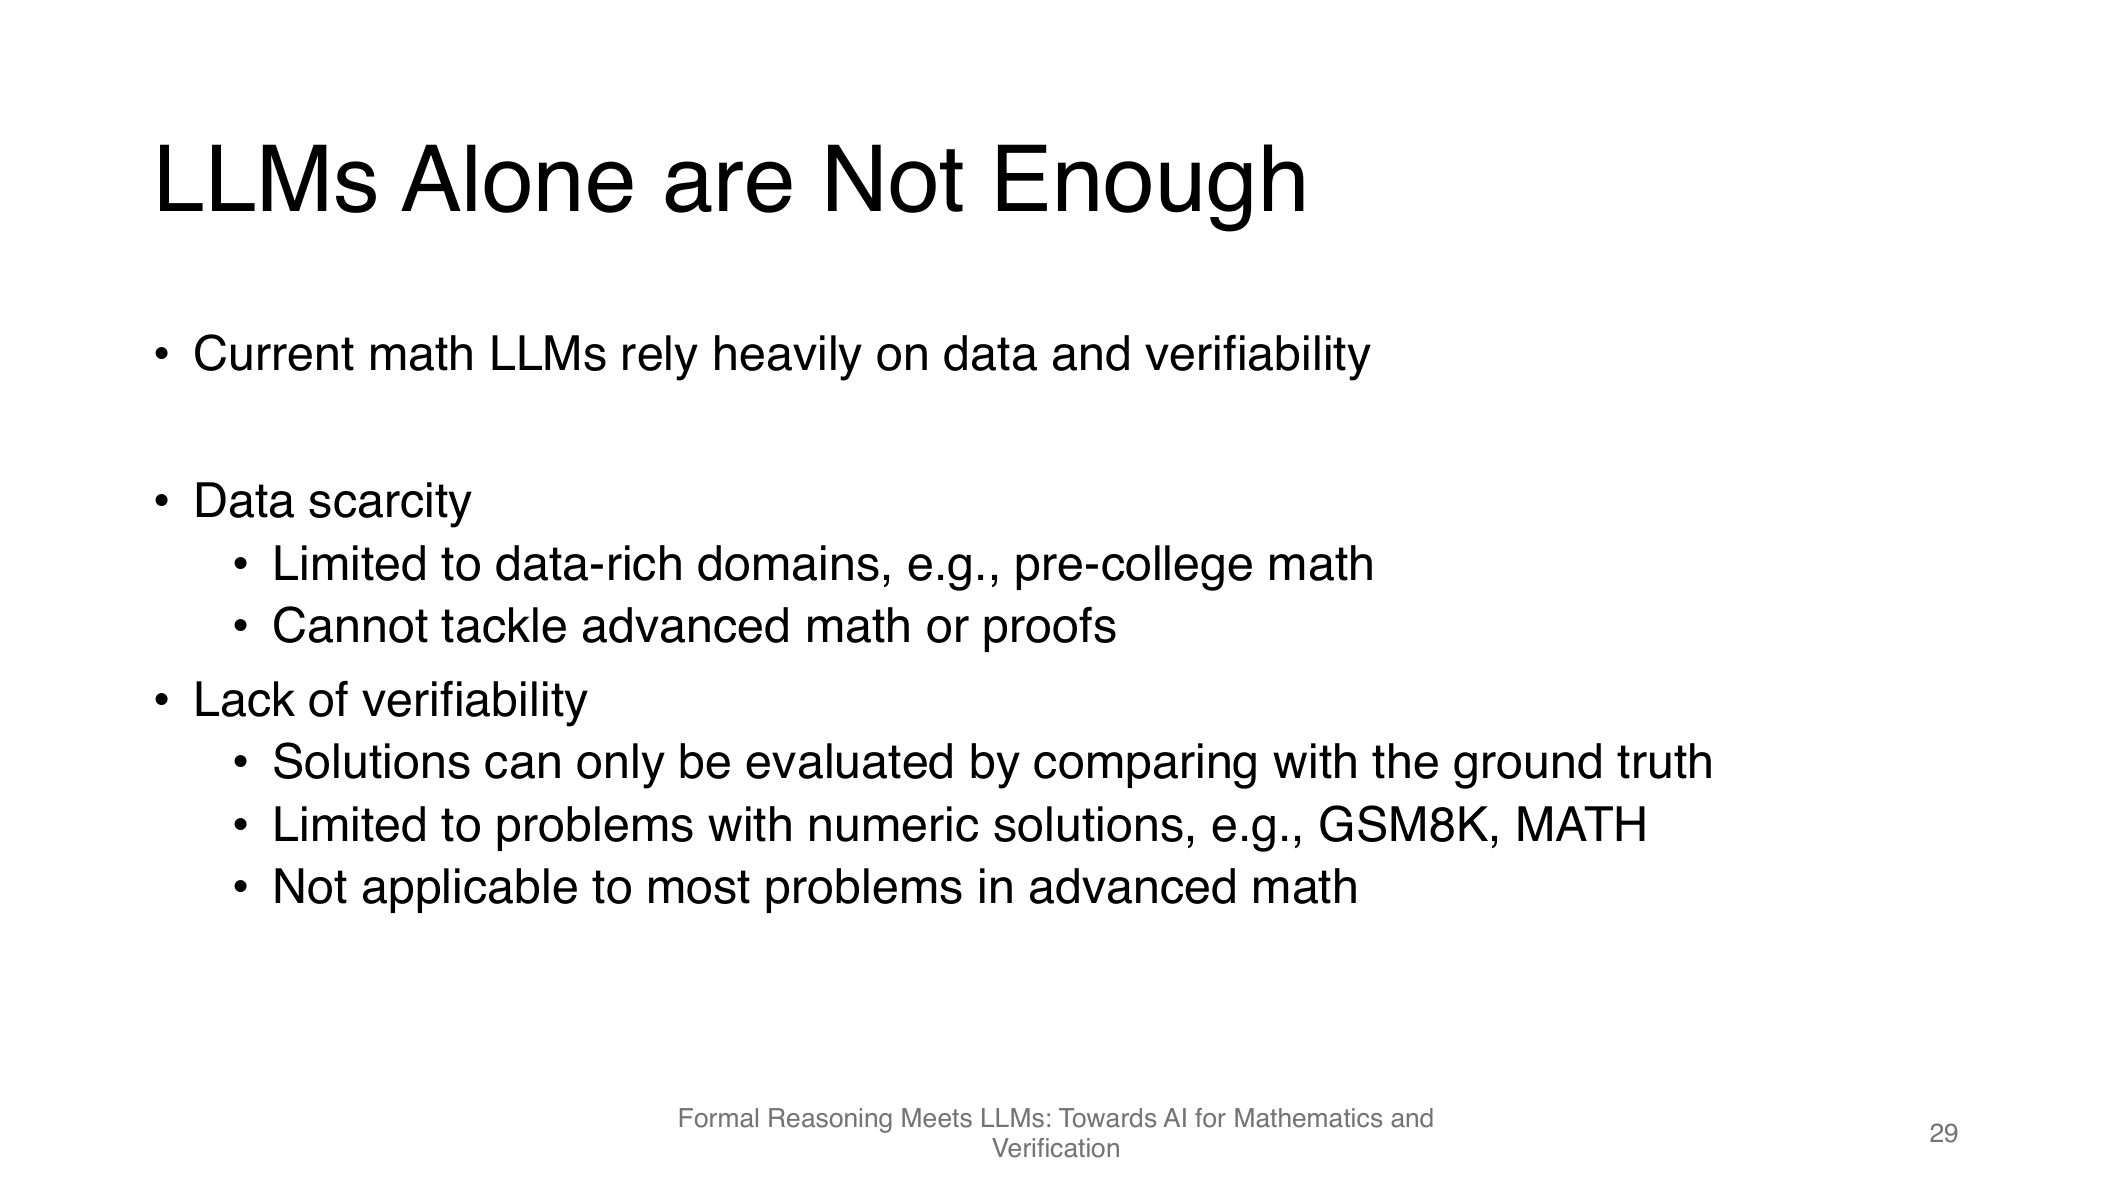
\includegraphics[width=0.80\textwidth]{figures/lec09_fig_003.png}
\caption{仅靠 LLM 文本能力仍然不够。}
\end{figure}

这也是讲者为什么强调 \textbf{formal reasoning is the missing ingredient}。formal reasoning 把数学从“可被文字描述的任务”改写成“可在 formal system 中被检查和搜索的任务”。这一步与 L08 的 AlphaProof 正好对上：若没有 formal environment，RL 和 search 很难得到可靠反馈；若没有 theorem-proving machinery，formal environment 又只会停留在静态库。

\section{核心概念与术语}

\begin{itemize}
\item \textbf{informal reasoning}：自然语言层面的数学解释、草图和启发式推理，允许大量默认背景知识。
\item \textbf{formal specification}：把问题写成 proof assistant 能接受的 formal theorem statement 或 program specification。
\item \textbf{verification}：让 proof checker 或 verifier 判断一条 formal proof / program trace 是否满足规范。
\item \textbf{theorem proving}：在形式系统内部构造证明，输出的是 formal proof steps 或 tactics。
\item \textbf{proof search}：在 proof states 与 actions 的图上进行系统探索，可能结合 retrieval、pruning、value estimates 或 symbolic rules。
\item \textbf{autoformalization}：从 informal theorem 或 informal proof 自动翻译出 formal theorem 或 formal proof。
\end{itemize}

\begin{knowledgebox}{不要把这些术语压扁成“数学推理”}
verification 负责检查，formal specification 负责把对象写对，autoformalization 负责自动生成 formal 表示，theorem proving 负责在 formal system 中找证明，proof search 则是 theorem proving 的算法内核。它们相关，但不能互相替代。
\end{knowledgebox}

\section{formal reasoning 的环境视角}

\subsection{proof assistants：为什么它们是 agent environment}

讲者把 proof assistant 定义为“用于书写 formal math 和 formal software proofs 的编程语言”。这一定义非常重要，因为它说明 formal reasoning 不是纯文本任务，而是\textbf{在程序化环境中操作形式对象}。

\begin{figure}[H]
\centering
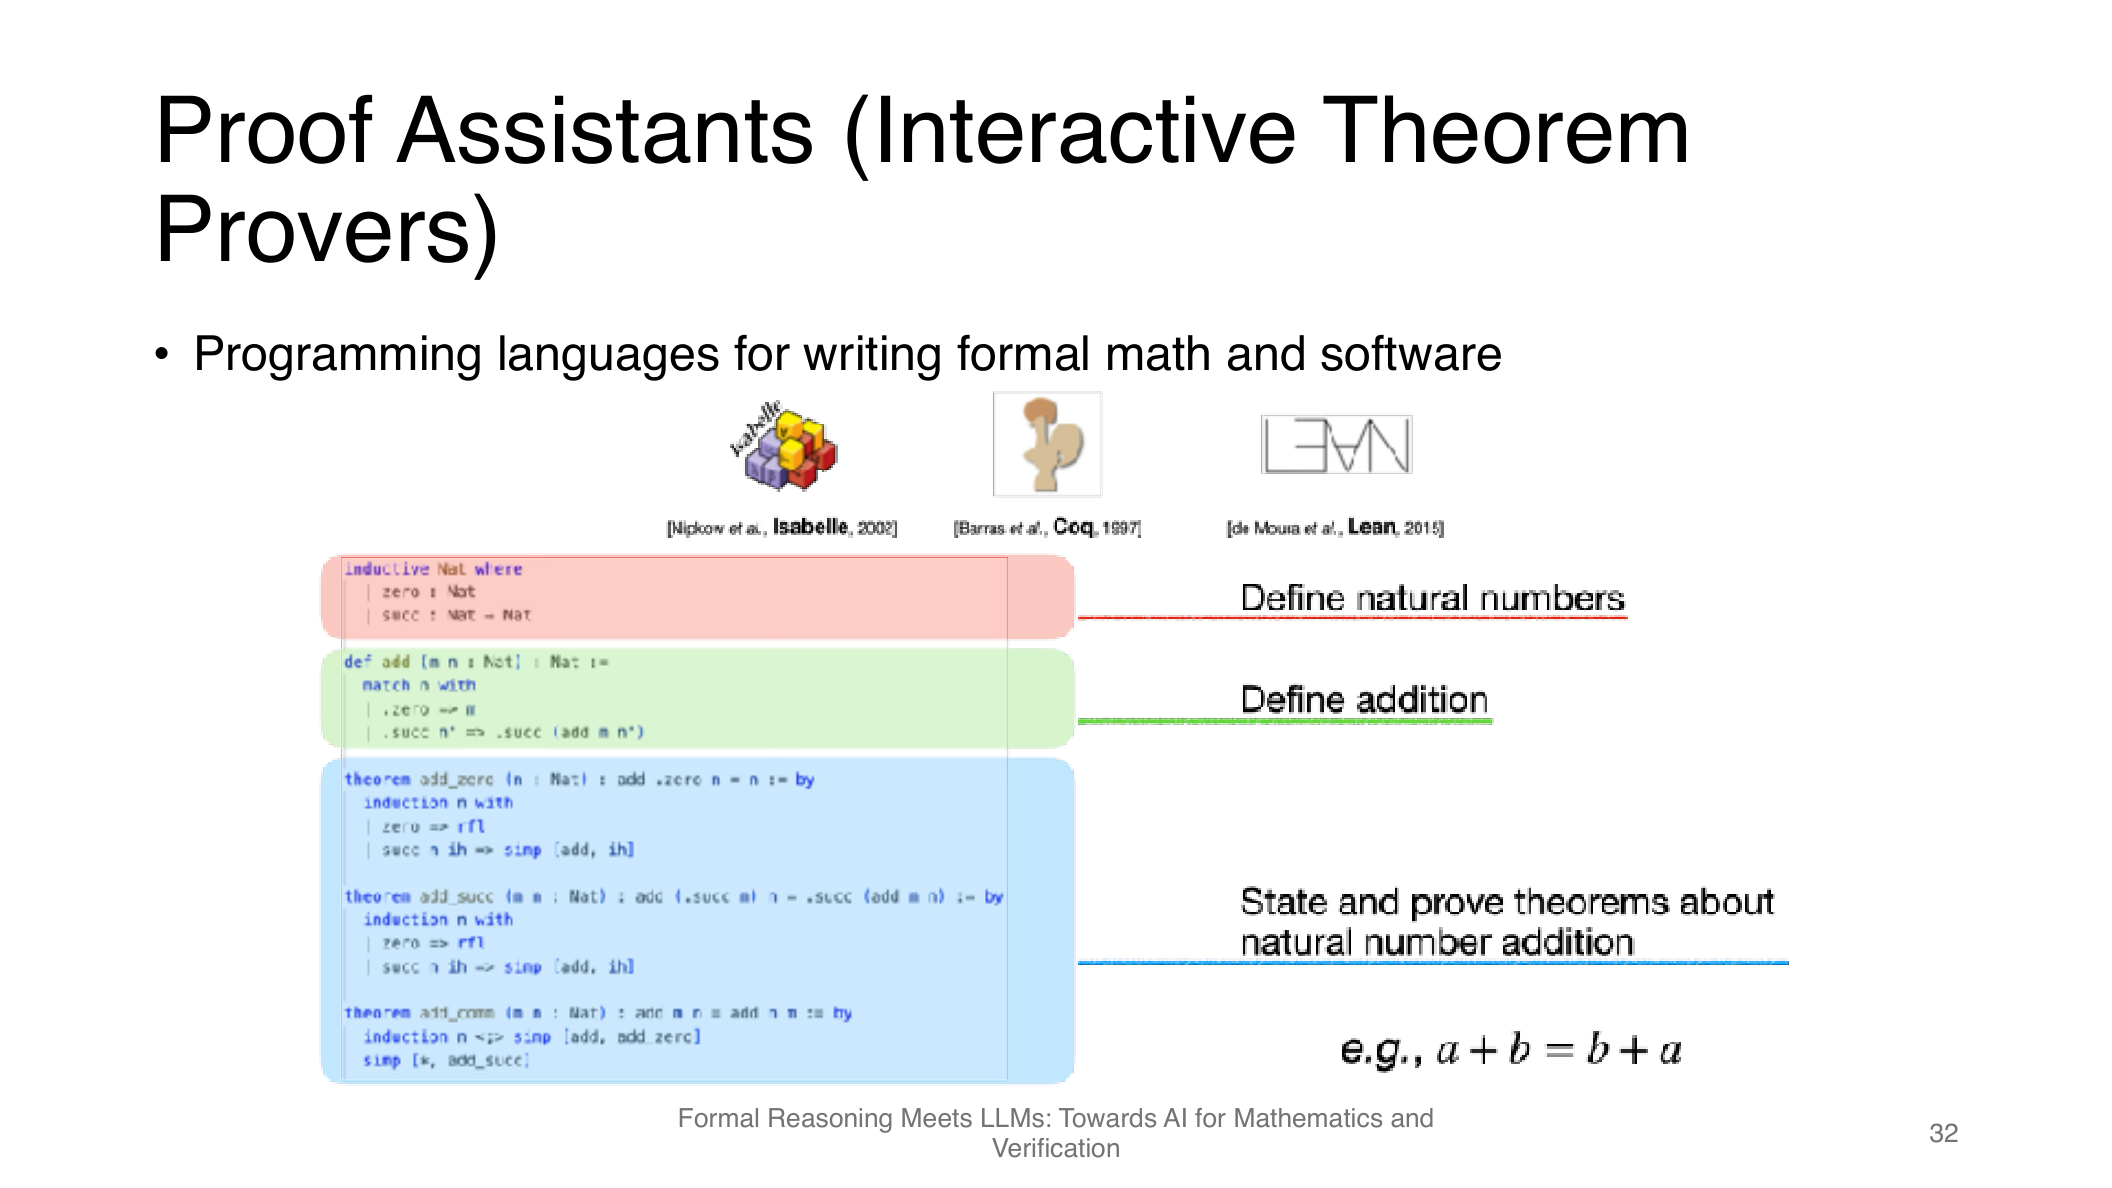
\includegraphics[width=0.78\textwidth]{figures/lec09_fig_004.png}
\caption{Proof assistant 是 formal reasoning 的执行环境。}
\end{figure}

在 Lean 中，定理、假设、proof state 和 tactics 都是显式对象。你不是在写一段让人“看起来像证明”的文字，而是在执行一系列状态转移，让 checker 最终接受目标。

\subsection{Lean proof state：从文本生成到交互式搜索}

\begin{figure}[H]
\centering
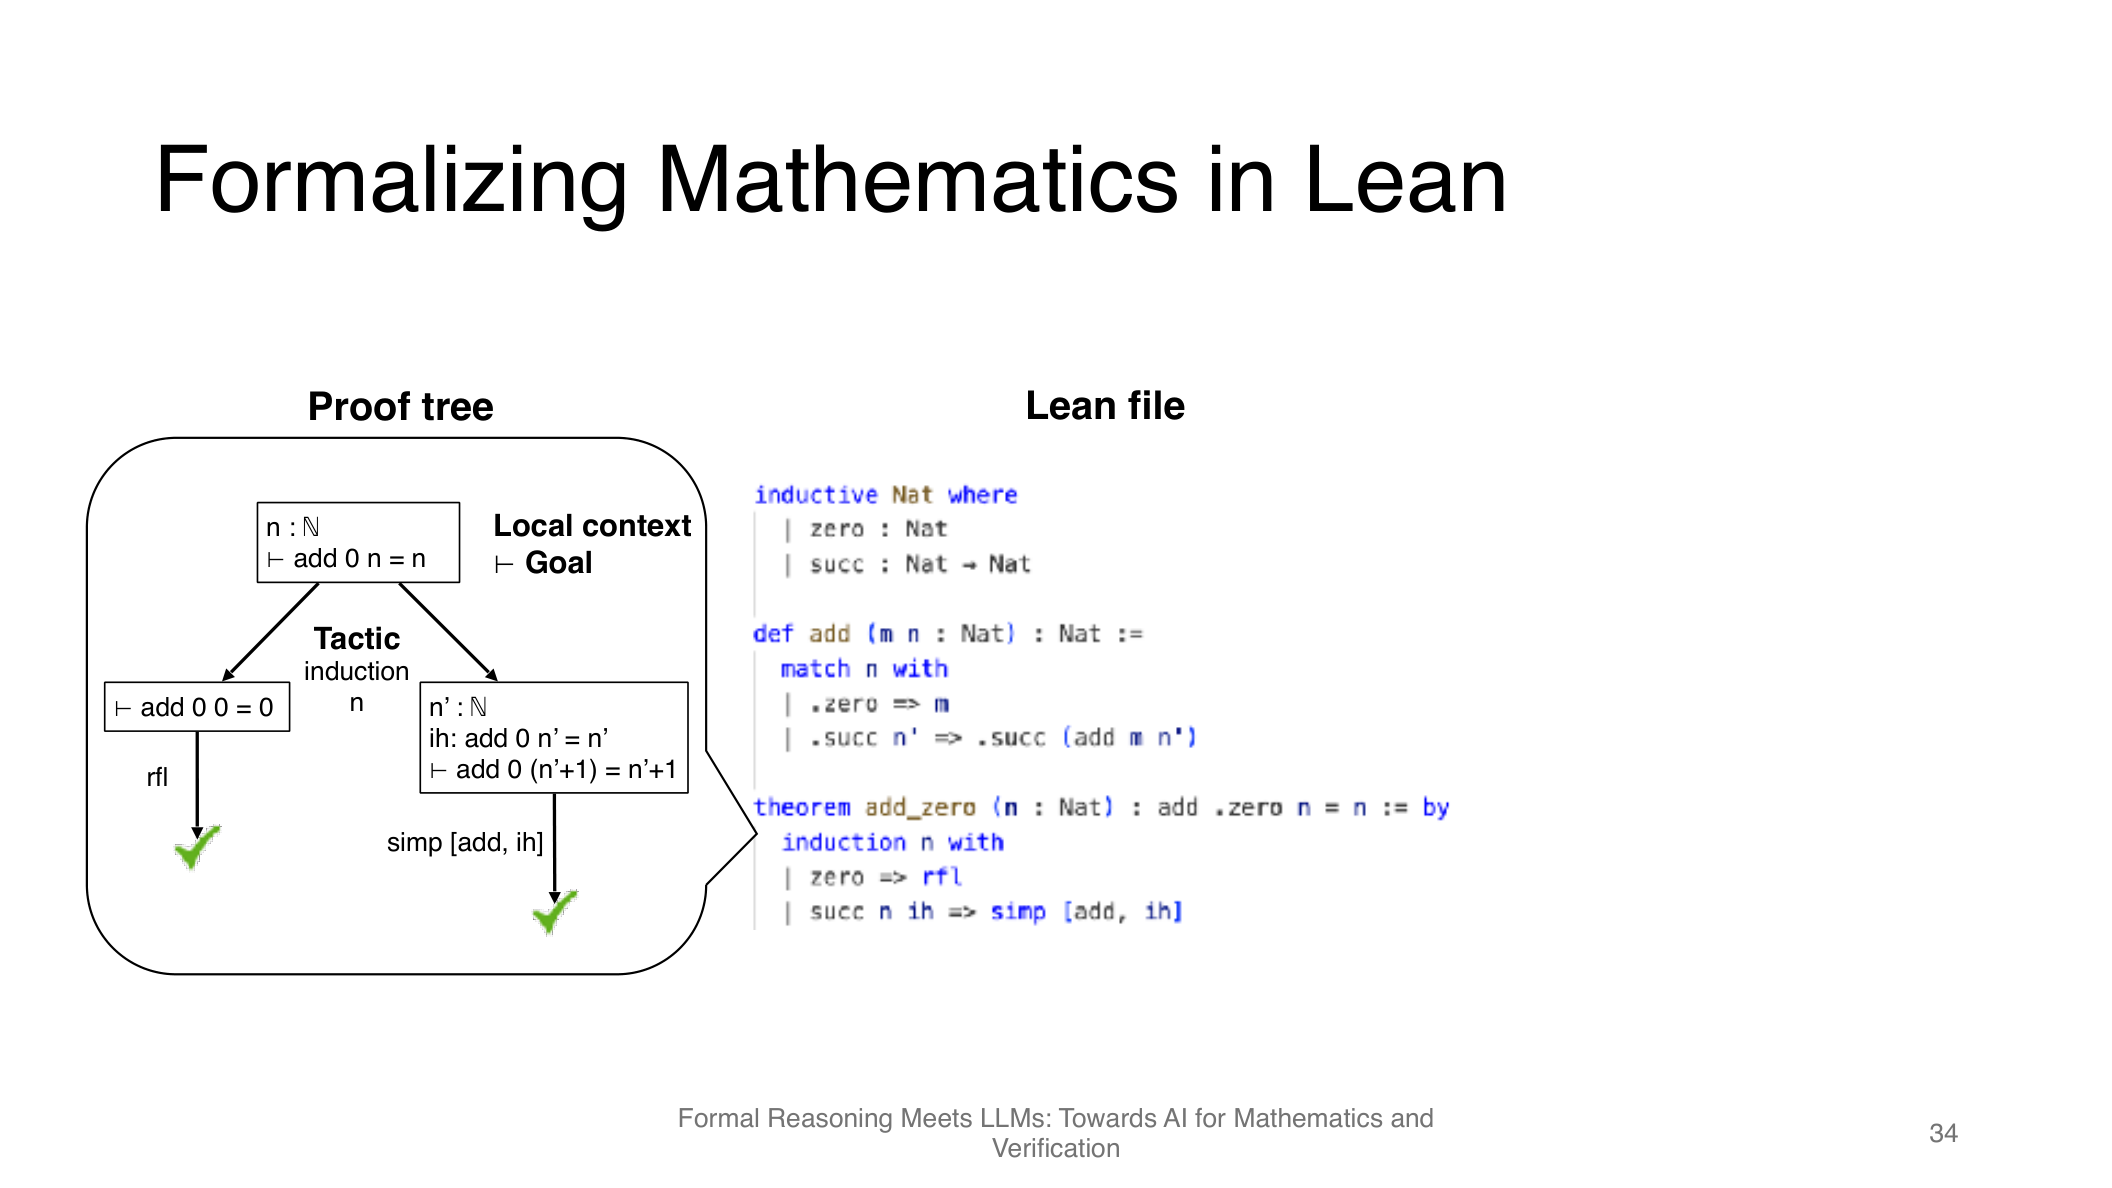
\includegraphics[width=0.80\textwidth]{figures/lec09_fig_005.png}
\caption{Lean proof state 将 theorem proving 具体化为 state transition。}
\end{figure}

这正是 theorem proving 与普通 math QA 的本质差别。一个典型交互循环是：

\begin{lstlisting}
while goals remain:
    inspect the current Lean proof state
    generate one or more tactics
    execute a tactic in Lean
    keep the next state if Lean accepts it; otherwise backtrack
\end{lstlisting}

这里已经能看出几层角色划分：
\begin{itemize}
\item \textbf{verification}：Lean 判断 tactic 合不合法。
\item \textbf{theorem proving}：找到能让 goals 全部消失的 tactic sequence。
\item \textbf{proof search}：在多条 tactic sequences 之间做探索、回溯和评分。
\end{itemize}

\subsection{L08 的 AlphaProof 在本讲中的位置}

\begin{figure}[H]
\centering
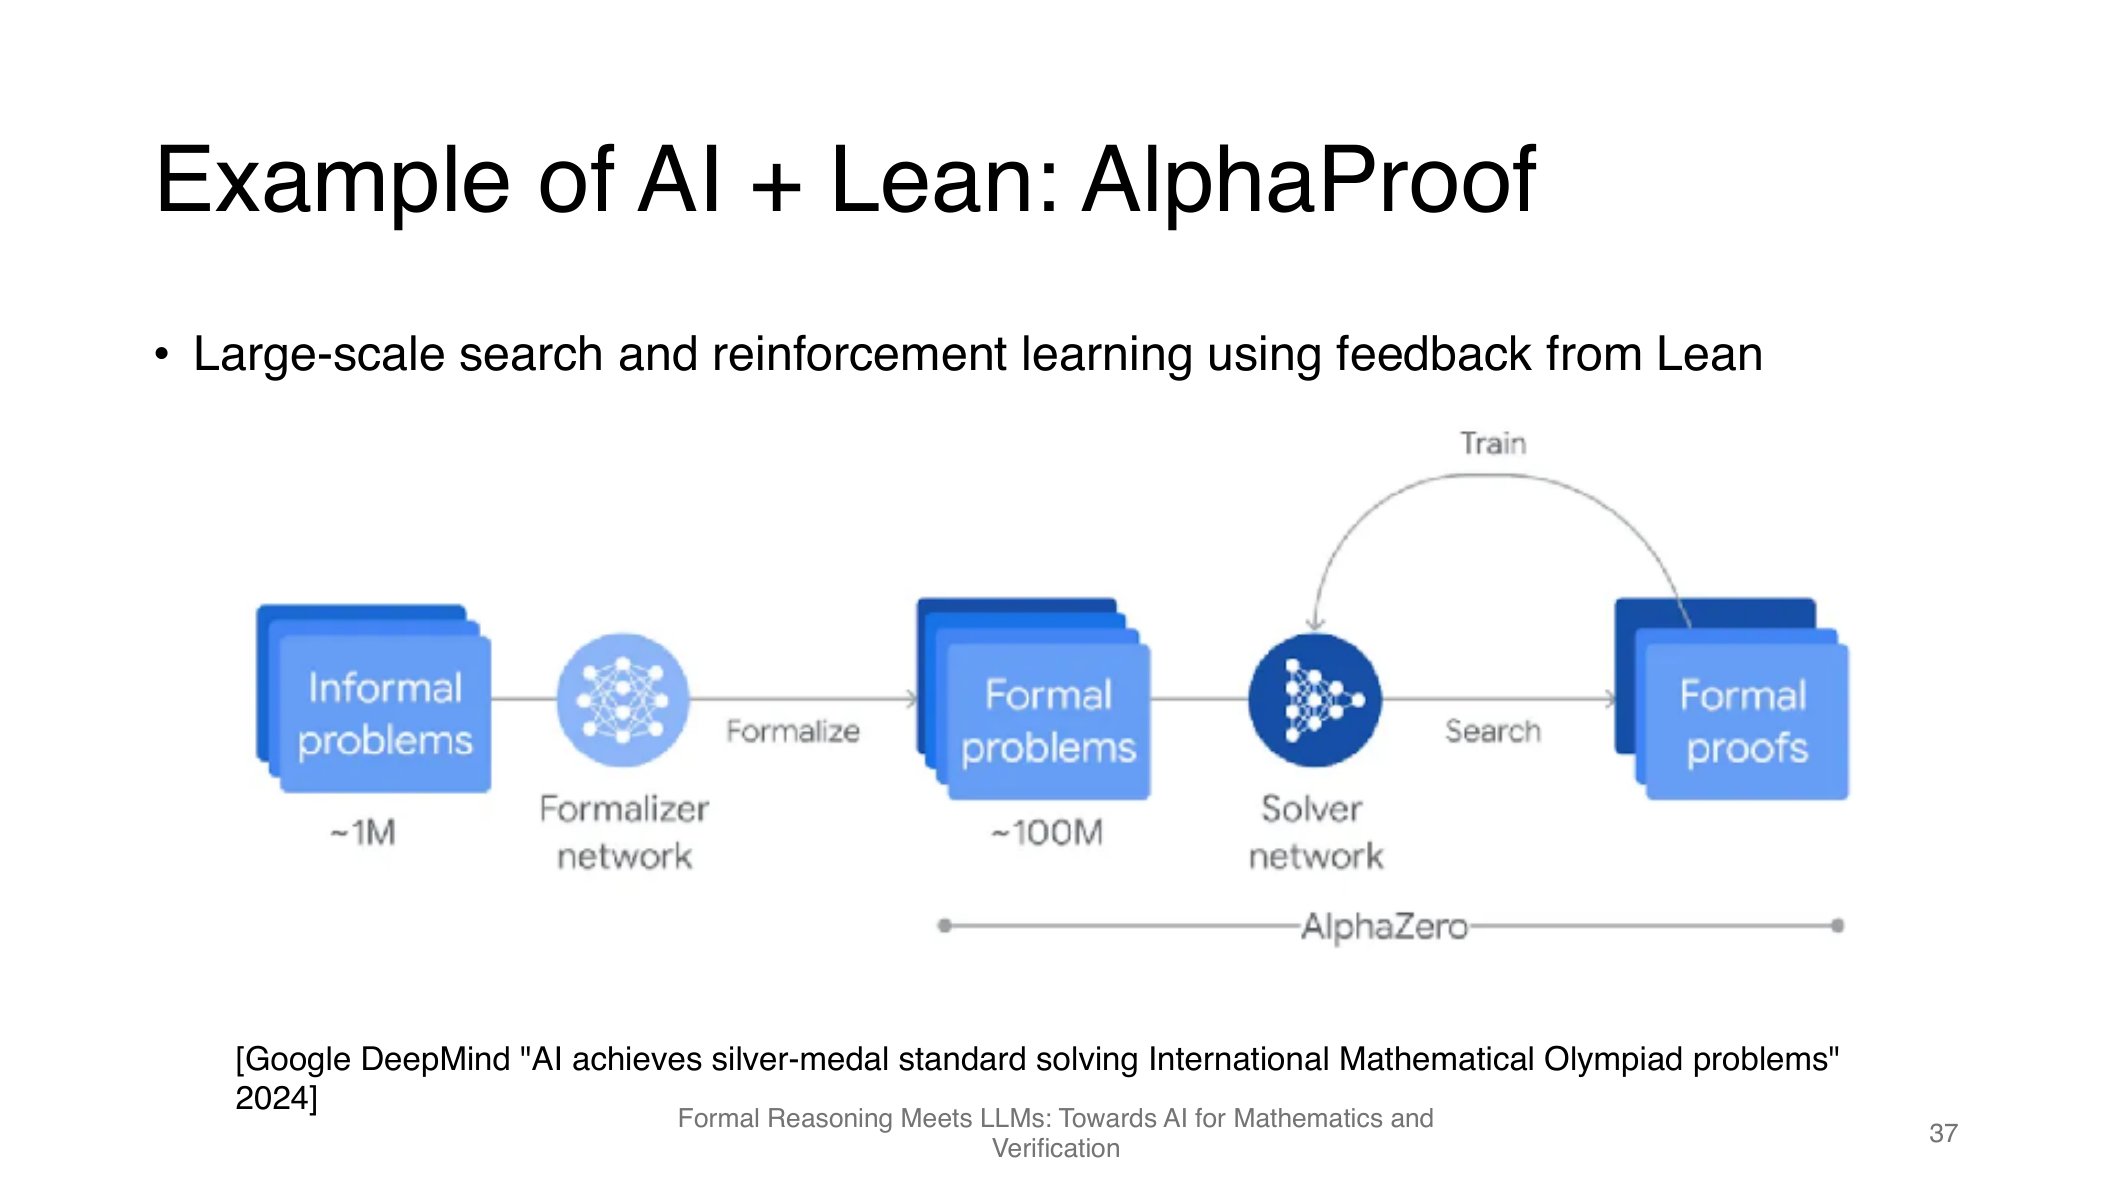
\includegraphics[width=0.78\textwidth]{figures/lec09_fig_006.png}
\caption{AlphaProof 作为 AI + Lean 的实例。}
\end{figure}

Kaiyu Yang 在这里把 AlphaProof 放进更大的 taxonomy 中：它说明 theorem proving 可以和 RL 深度耦合，但也同时暴露出 formalization 与 domain coverage 的问题。因此 L08 可以被看作“formal reasoning 环境可行”的系统论证，而 L09 更像“formal reasoning 任务族如何拆解”的方法论讲义。

\section{theorem proving：从开放基础设施到检索增强系统}

\subsection{LeanDojo：把 theorem proving 研究变成可复现工程}

LeanDojo 的价值首先不在模型，而在基础设施。它把 Lean 中的 theorem/proof 数据、premise annotations、benchmark split 和 programmatic interaction 一次性开放出来，从而把 theorem proving 从“只有少数大实验室能做的私有工程”变成可复现研究问题。

\begin{figure}[H]
\centering
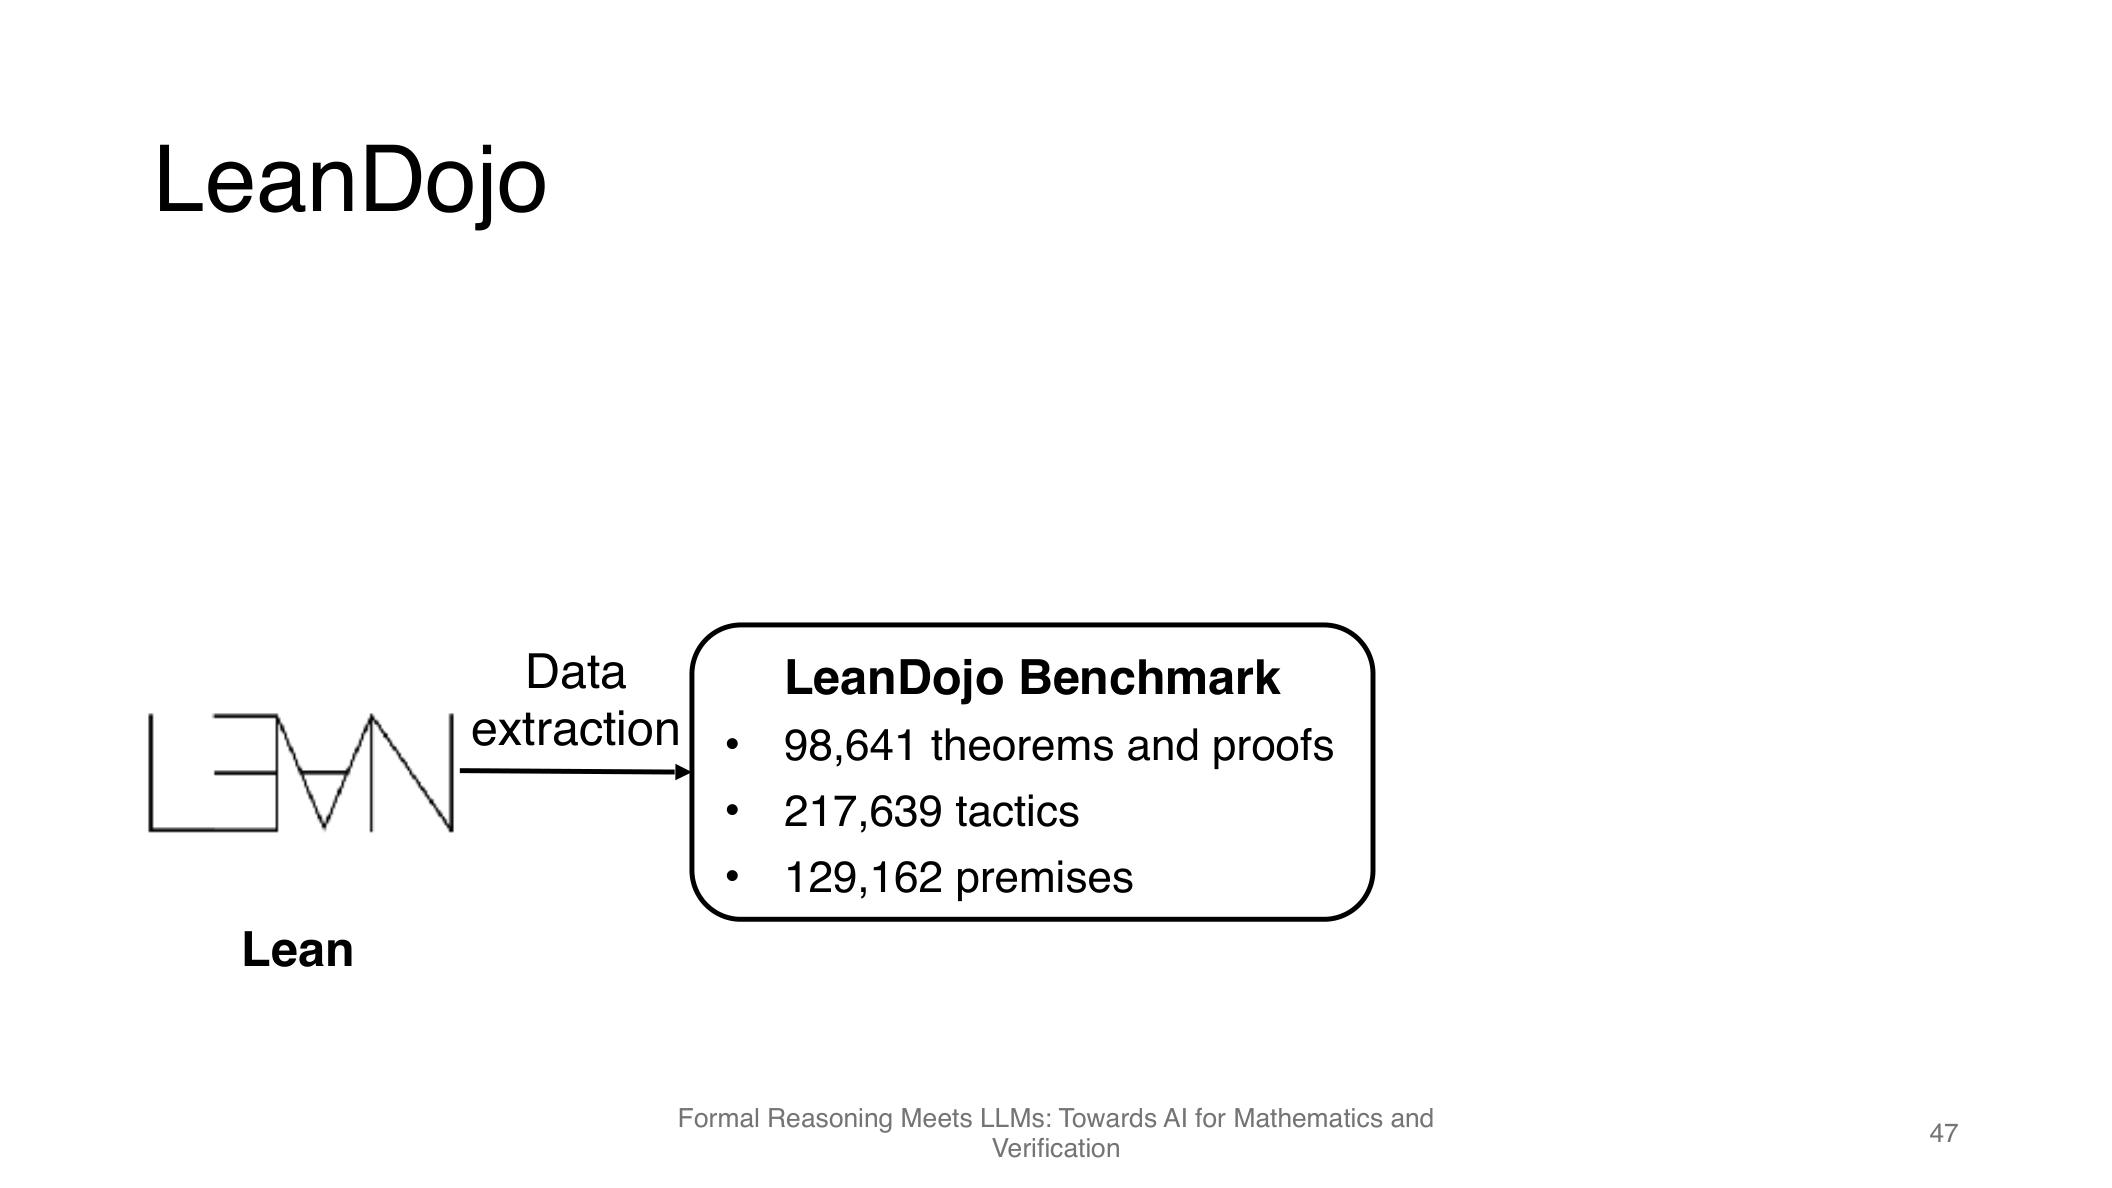
\includegraphics[width=0.84\textwidth]{figures/lec09_fig_007.png}
\caption{LeanDojo benchmark 的数据规模与开放接口。}
\end{figure}

这与 harness engineering 的精神完全一致：环境、数据、检查器和交互接口必须先被组织好，agent 才有机会稳定迭代。LeanDojo 做的正是 theorem proving 版本的“repo as record system”。

\subsection{ReProver：为什么 theorem proving 需要 retrieval}

\begin{figure}[H]
\centering
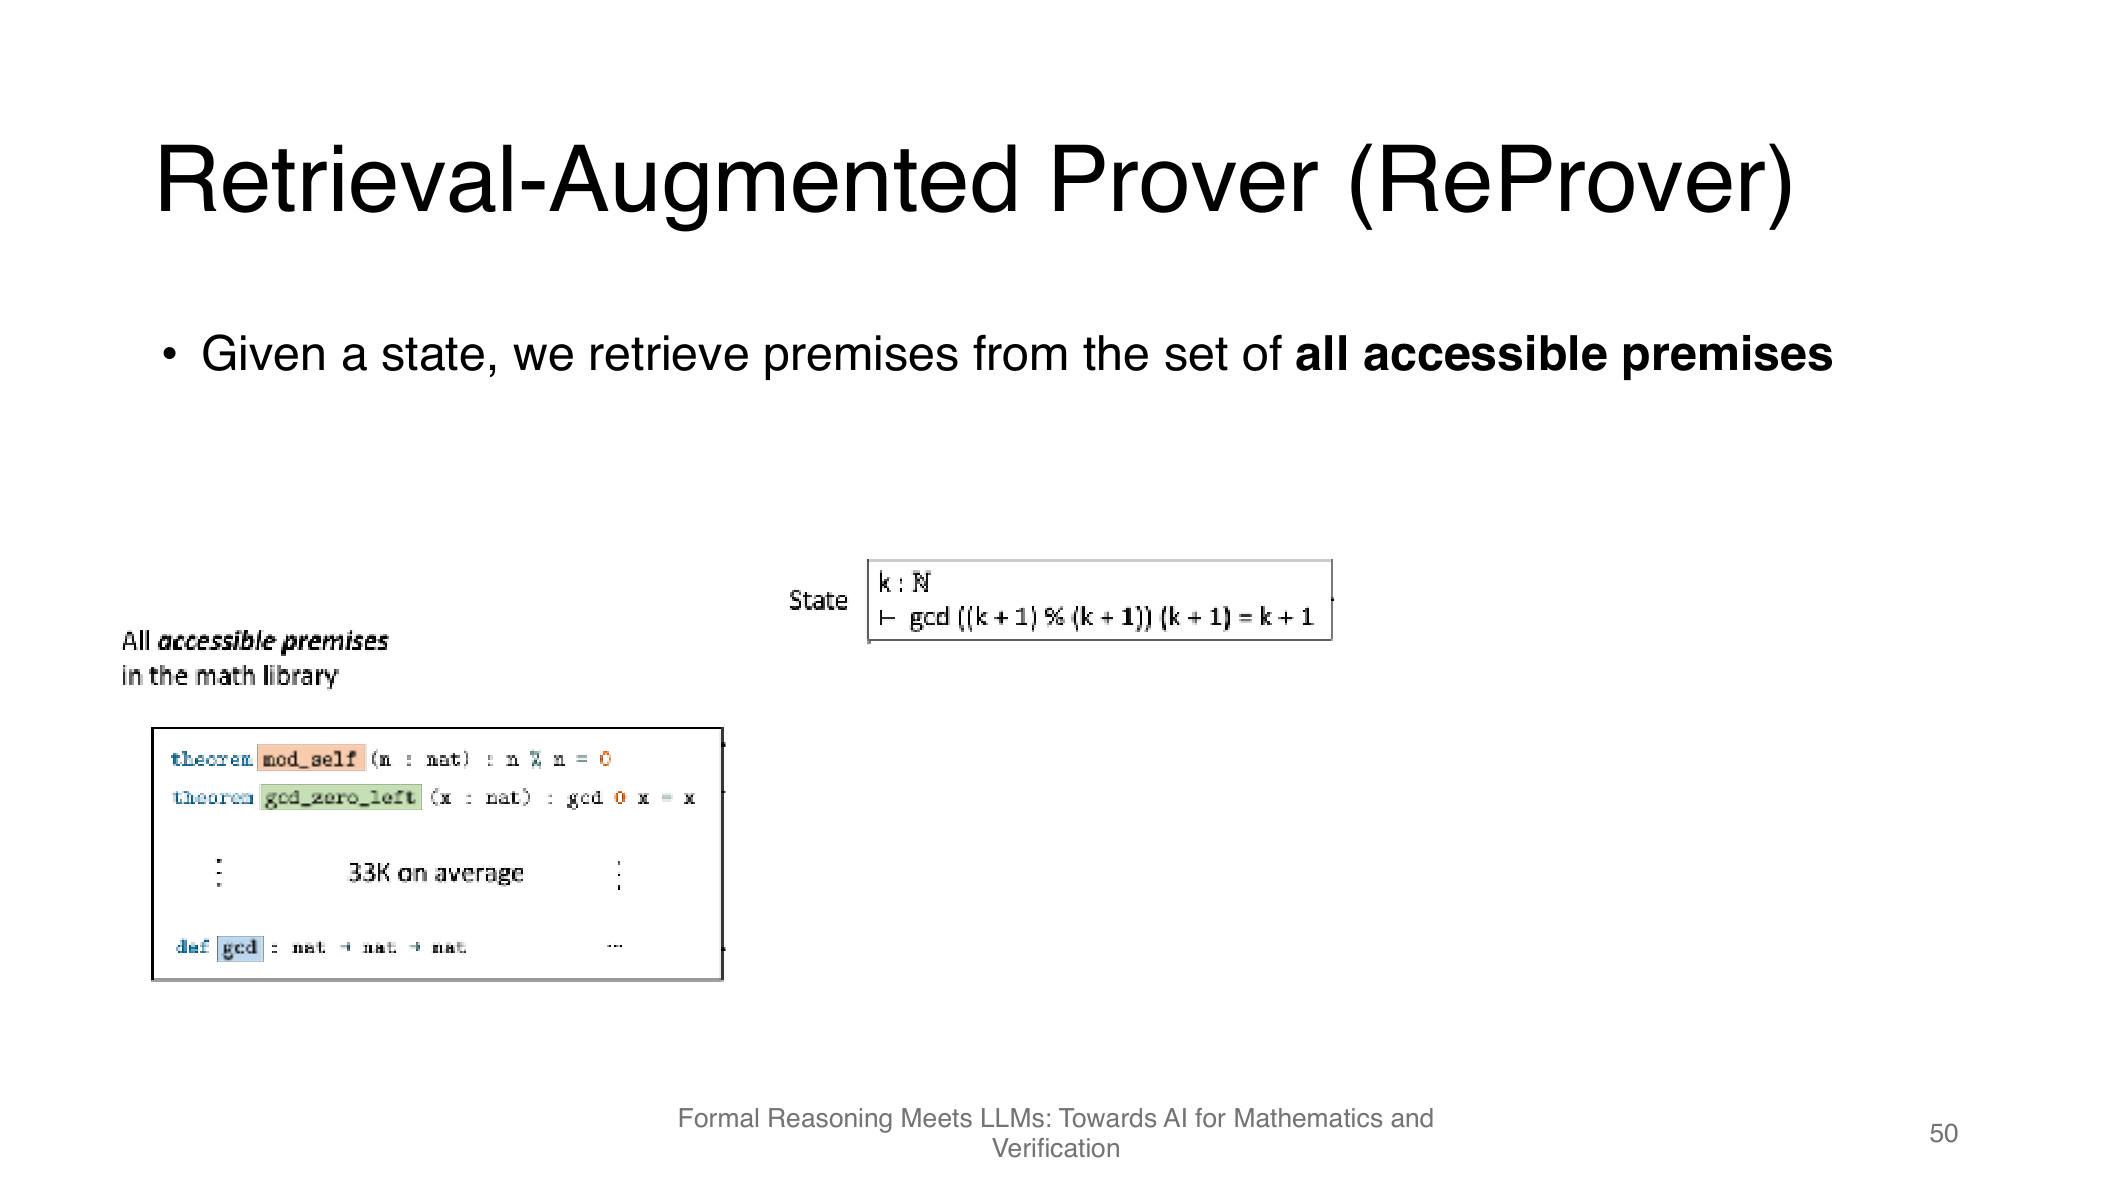
\includegraphics[width=0.84\textwidth]{figures/lec09_fig_008.png}
\caption{ReProver 的 retrieval-augmented proving。}
\end{figure}

给定当前 proof state $s$，ReProver 不会盲目生成 tactic，而是先在可访问 premises 集合中做检索，再结合检索结果生成下一步。这可抽象为
\[
(a^{\star}, P^{\star}) = \arg\max_{a, P}\; s_{\theta}(a \mid s, P) + \lambda\, r_{\eta}(P \mid s).
\]
其中 $P$ 是检索到的 premises，$s_{\theta}$ 是 tactic generation score，$r_{\eta}$ 是 retrieval score。直觉很简单：\textbf{定理证明不是只在“下一 token”上做决策，而是在“应该引用什么知识”和“下一步做什么”上联合决策。}

\begin{lstlisting}
given proof state s:
    retrieve accessible premises P from LeanDojo
    score premises with a retriever
    condition the language model on s and top premises
    generate next tactics and verify them in Lean
\end{lstlisting}

\begin{figure}[H]
\centering
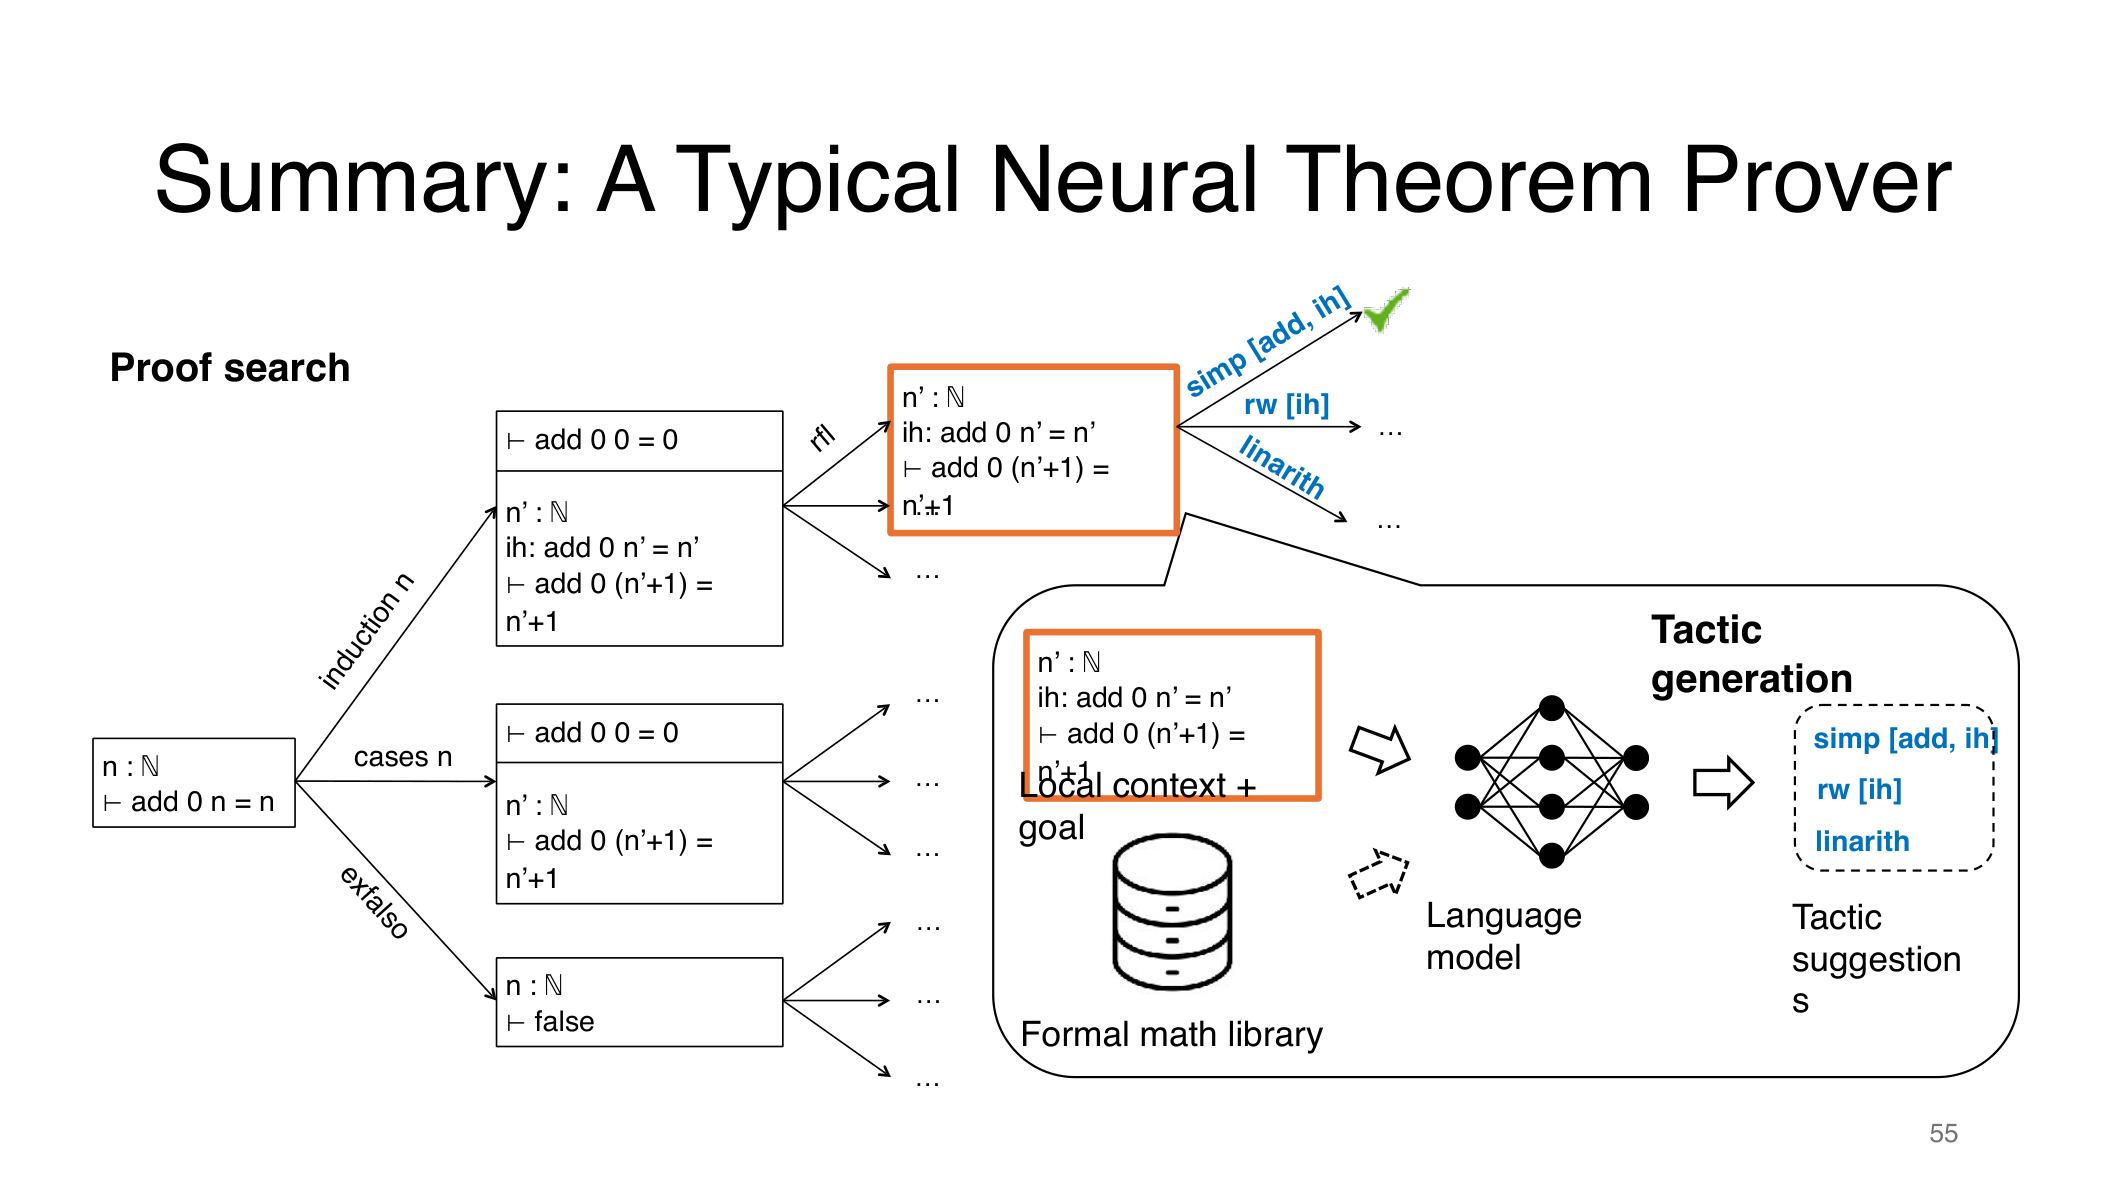
\includegraphics[width=0.84\textwidth]{figures/lec09_fig_009.png}
\caption{典型 neural theorem prover 是多模块系统。}
\end{figure}

这也是为什么“LLM 直接出 proof”通常不够。真正的系统至少还需要 premise access control、retrieval、search policy 和 checker feedback。

\subsection{infinite action space 与 LIPS 的启示}

\begin{figure}[H]
\centering
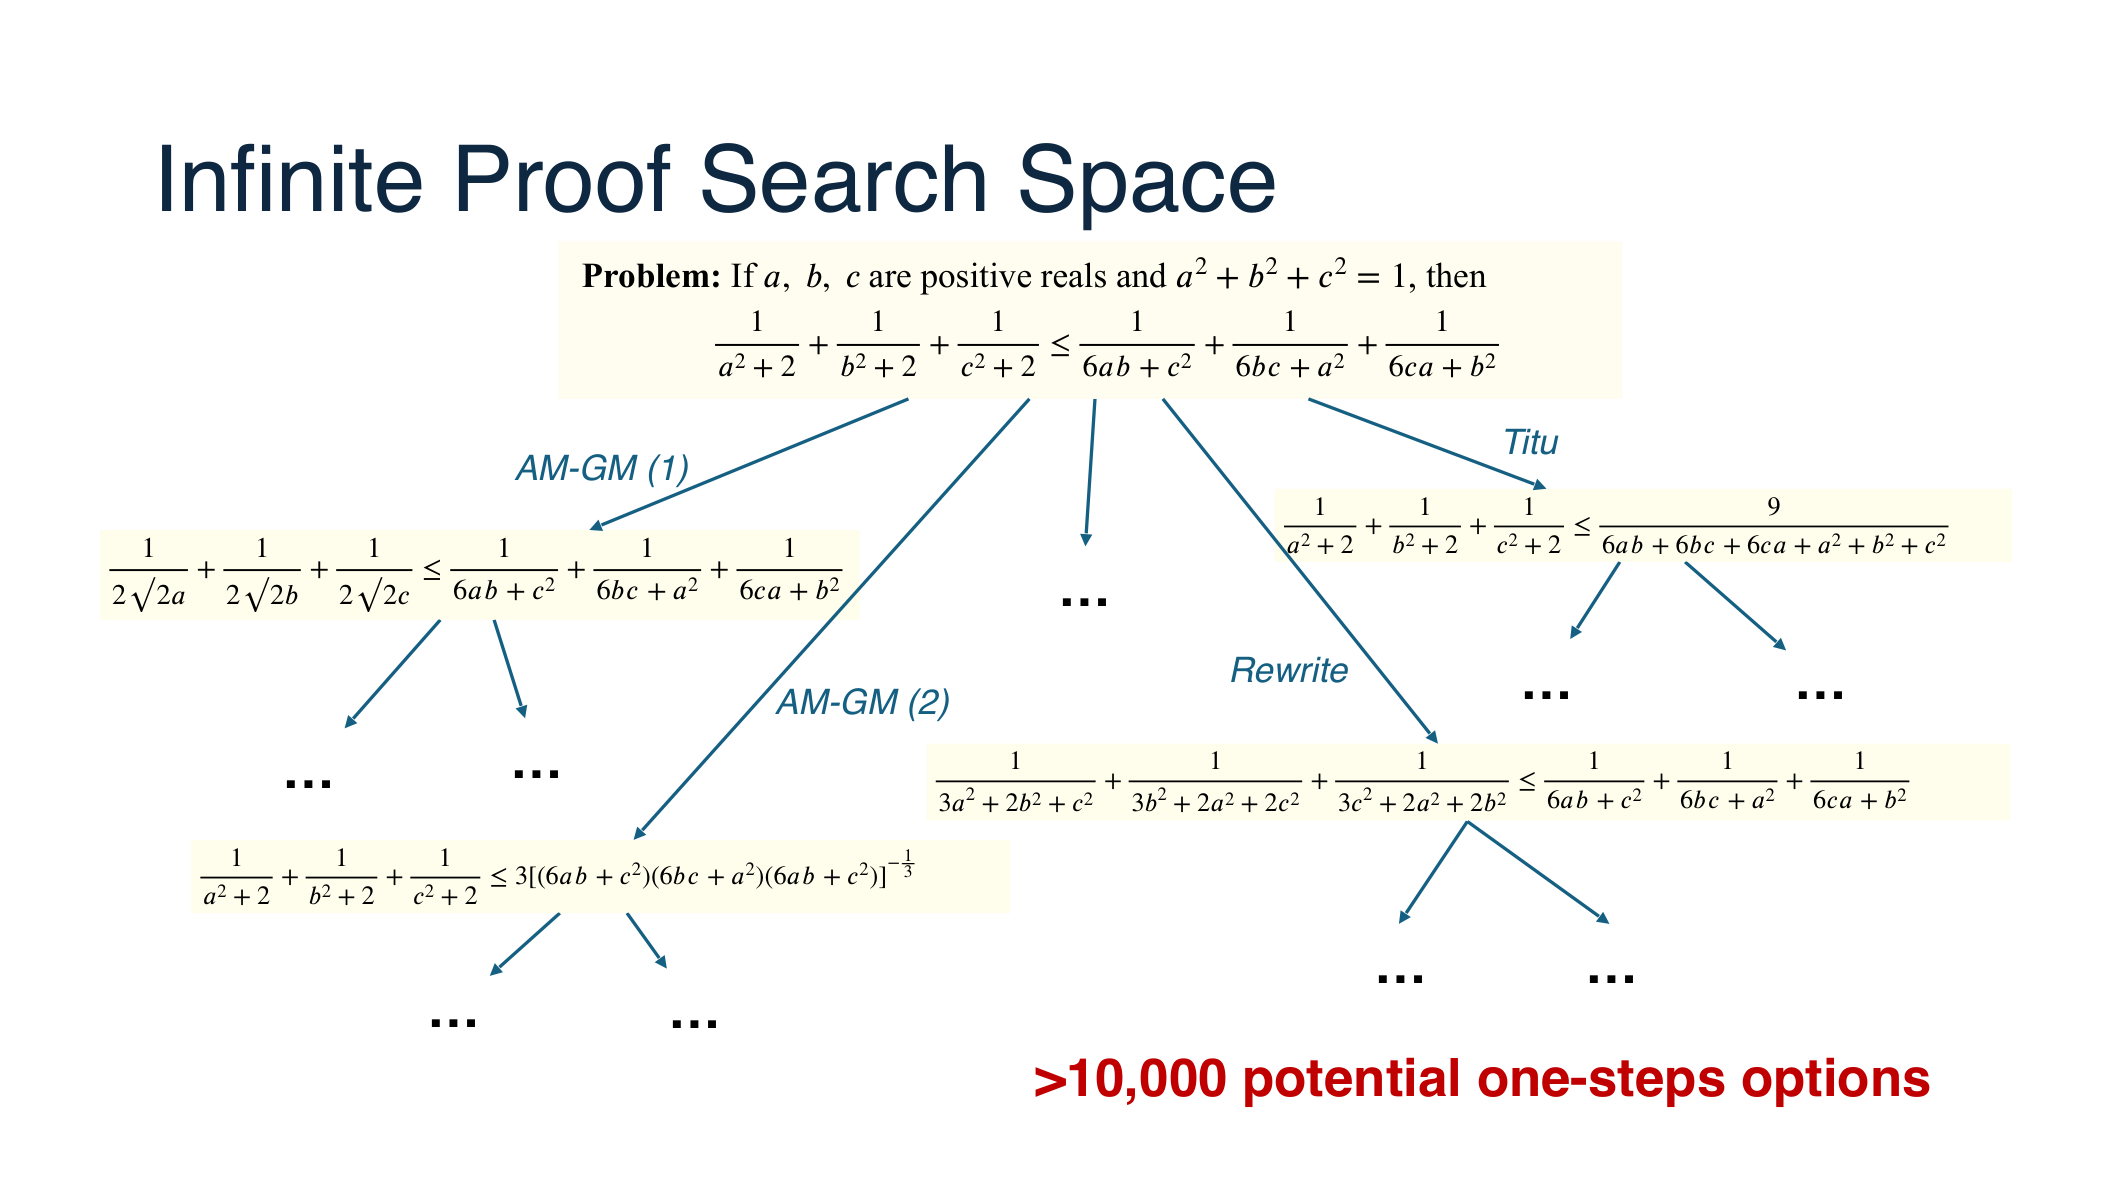
\includegraphics[width=0.82\textwidth]{figures/lec09_fig_010.png}
\caption{Theorem proving 的 action space 极大。}
\end{figure}

Slides 在 inequality proving 段落专门强调：proof search 的动作空间几乎是无限的。很多任务中，模型随时可以发明新的中间变换，而不是只从一个有限 action set 中选一项。这比棋类更接近开放规划问题。

\begin{figure}[H]
\centering
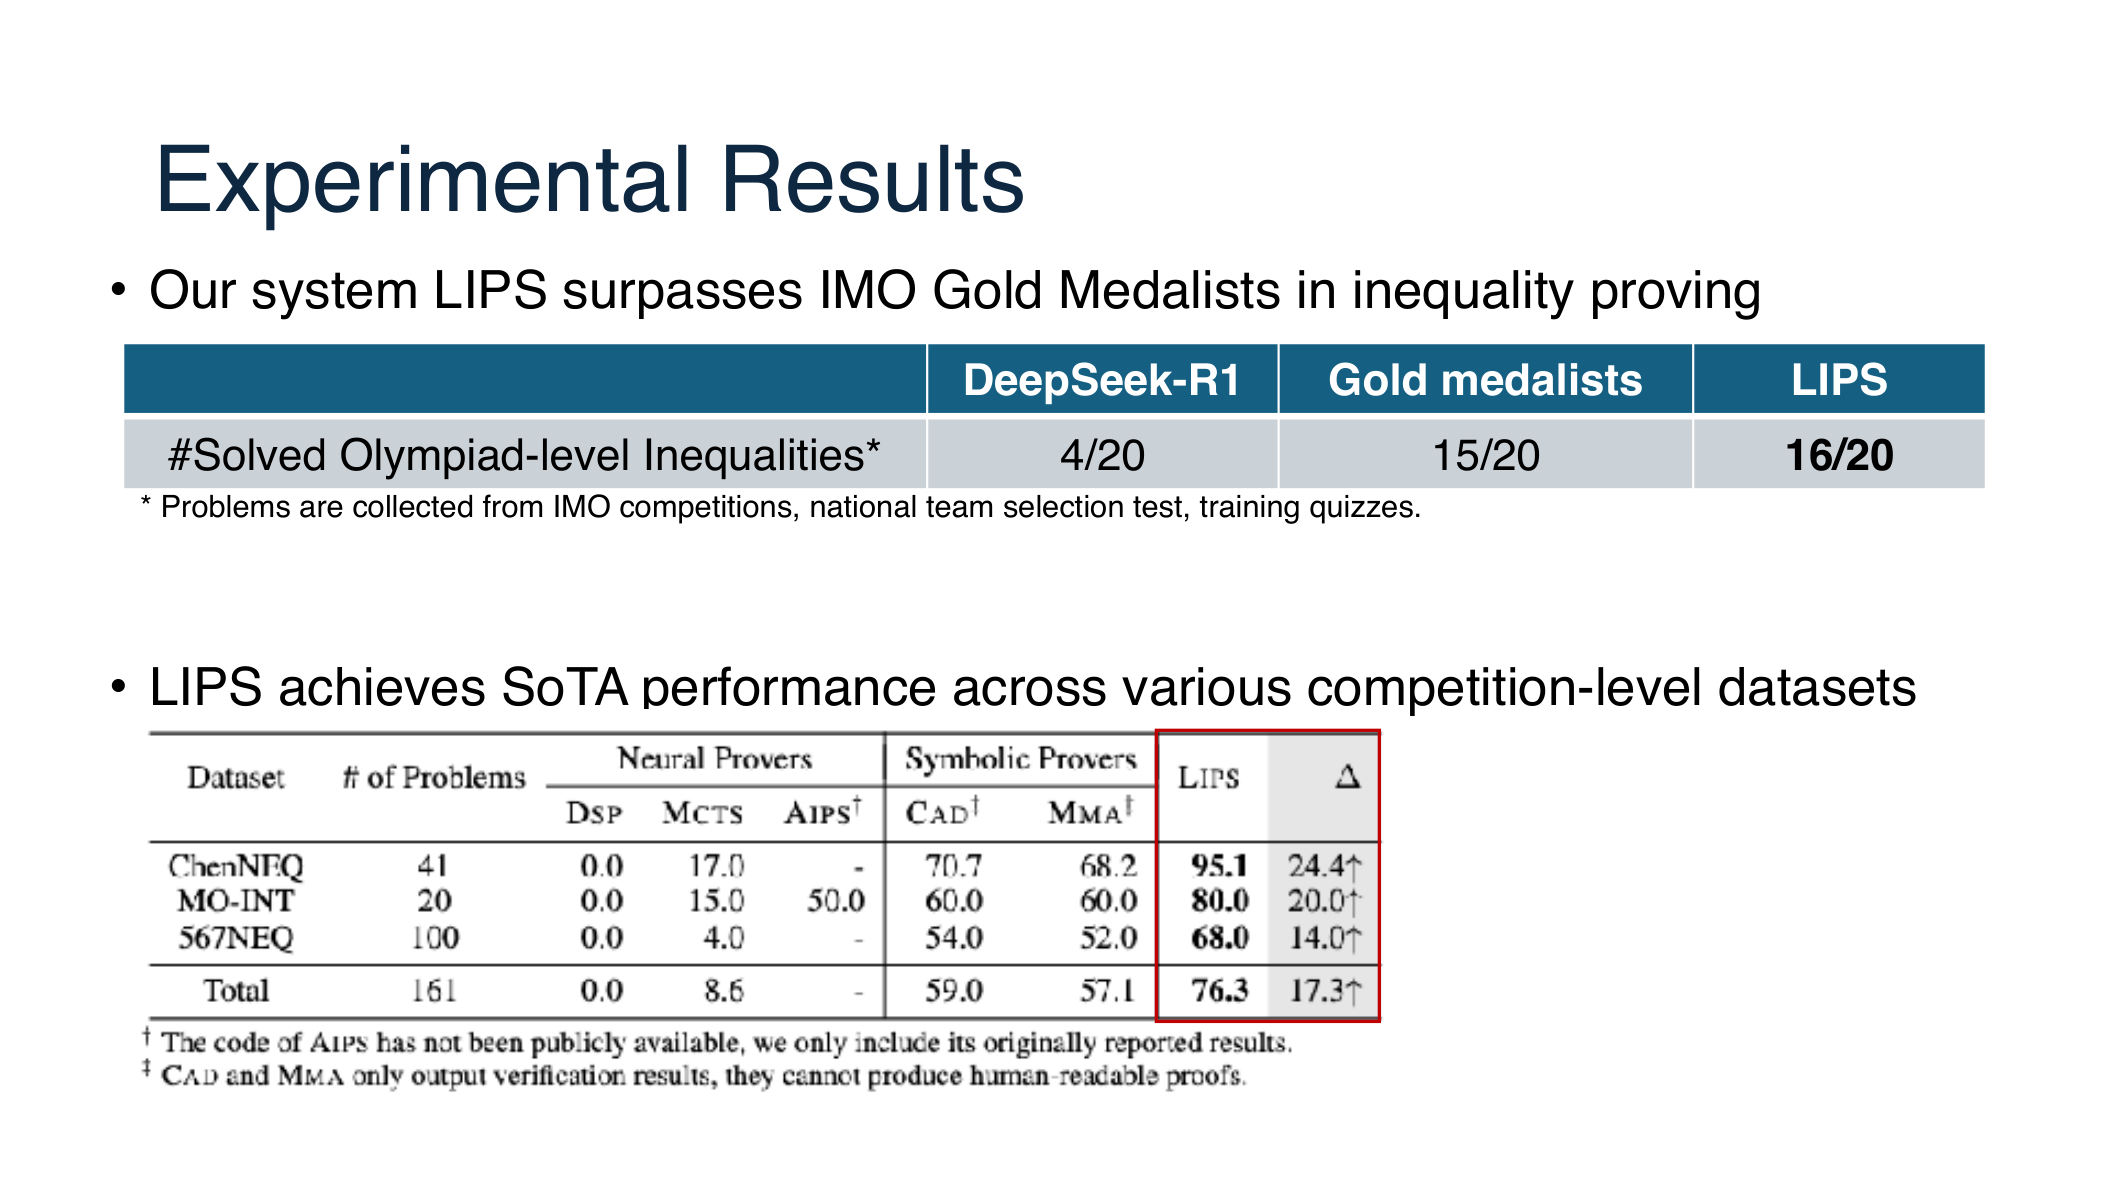
\includegraphics[width=0.82\textwidth]{figures/lec09_fig_011.png}
\caption{LIPS 的实验结果。}
\end{figure}

LIPS 给出的启示是：\textbf{如果某个子域有强结构，就应该把结构显式写进搜索。} 它通过把 inequality proving 的步骤分类、做 pruning，并结合符号推理来缩减搜索空间。换言之，通用大模型能力很重要，但 theorem proving 往往还需要 domain structure。

\begin{lstlisting}
generate algebraic transformations with an LLM
classify candidates as scaling or pruning steps
use symbolic checks to reject inconsistent branches early
continue search on the reduced proof space
\end{lstlisting}

\section{autoformalization：把 informal mathematics 送进 formal world}

\subsection{autoformalization 到底在做什么}

\begin{figure}[H]
\centering
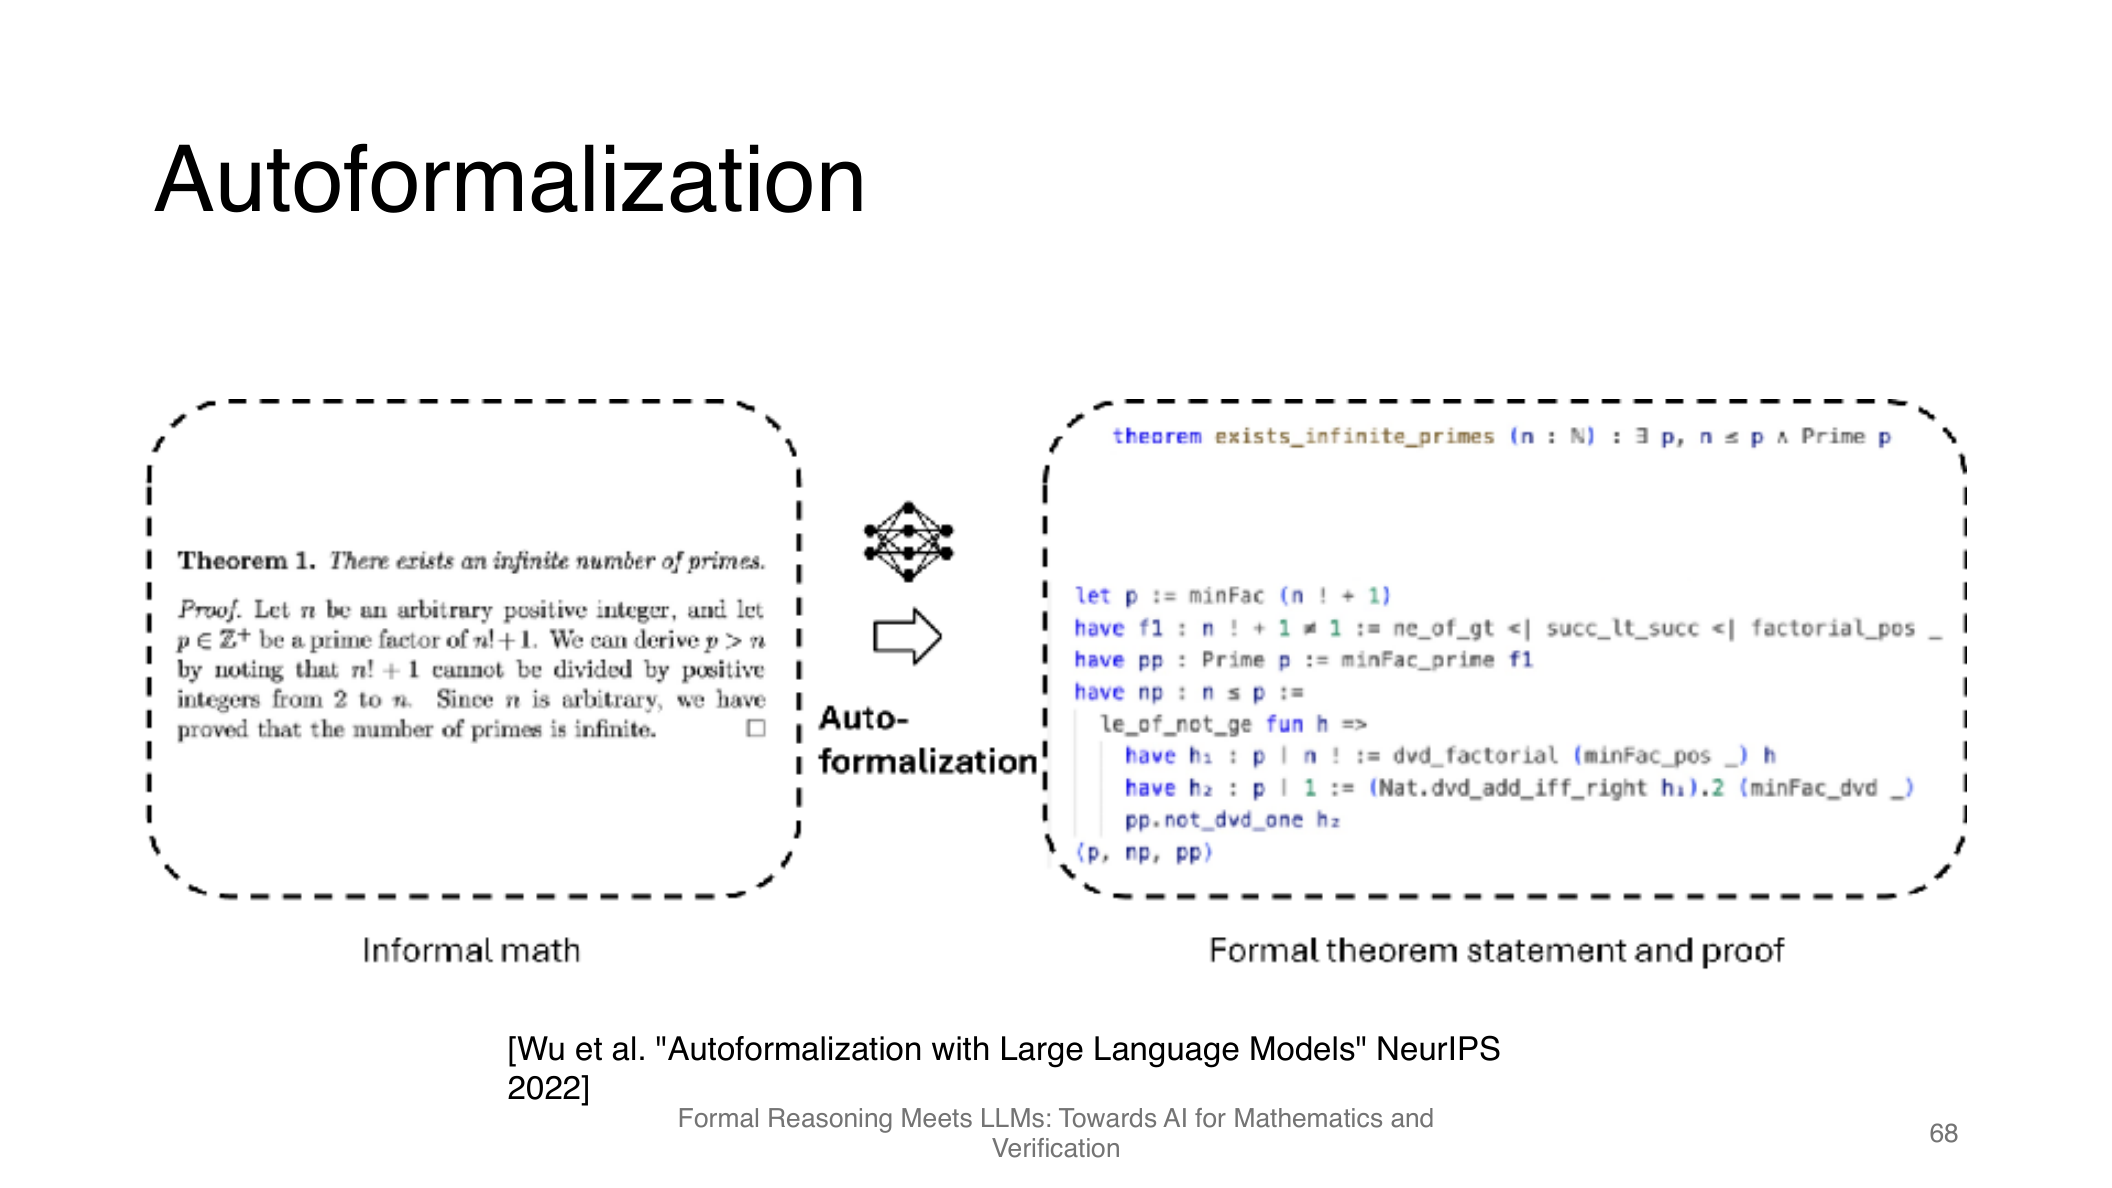
\includegraphics[width=0.80\textwidth]{figures/lec09_fig_012.png}
\caption{Autoformalization 的定义。}
\end{figure}

讲者把 autoformalization 拆成两类：theorem-level 和 proof-level。可抽象为
\[
\hat{T}_{\mathrm{formal}} = g_{\phi}(x_{\mathrm{informal}}), \qquad \hat{\pi}_{\mathrm{formal}} = h_{\psi}(x_{\mathrm{informal}}, T_{\mathrm{formal}}).
\]
第一项把自然语言 theorem 写成 formal statement；第二项把 informal proof 写成 formal proof。二者都不是 verification，也不是 theorem proving。它们是在构造 theorem prover 所需要的输入对象。

\begin{importantbox}{为什么这一步极其关键}
没有正确的 formal specification，再强的 theorem prover 也只是在错误问题上努力。autoformalization 决定了系统是否真正理解了原始题意，而不只是会在 formal system 里玩一个别的问题。
\end{importantbox}

\subsection{为什么 autoformalization 难以自动评估}

\begin{figure}[H]
\centering
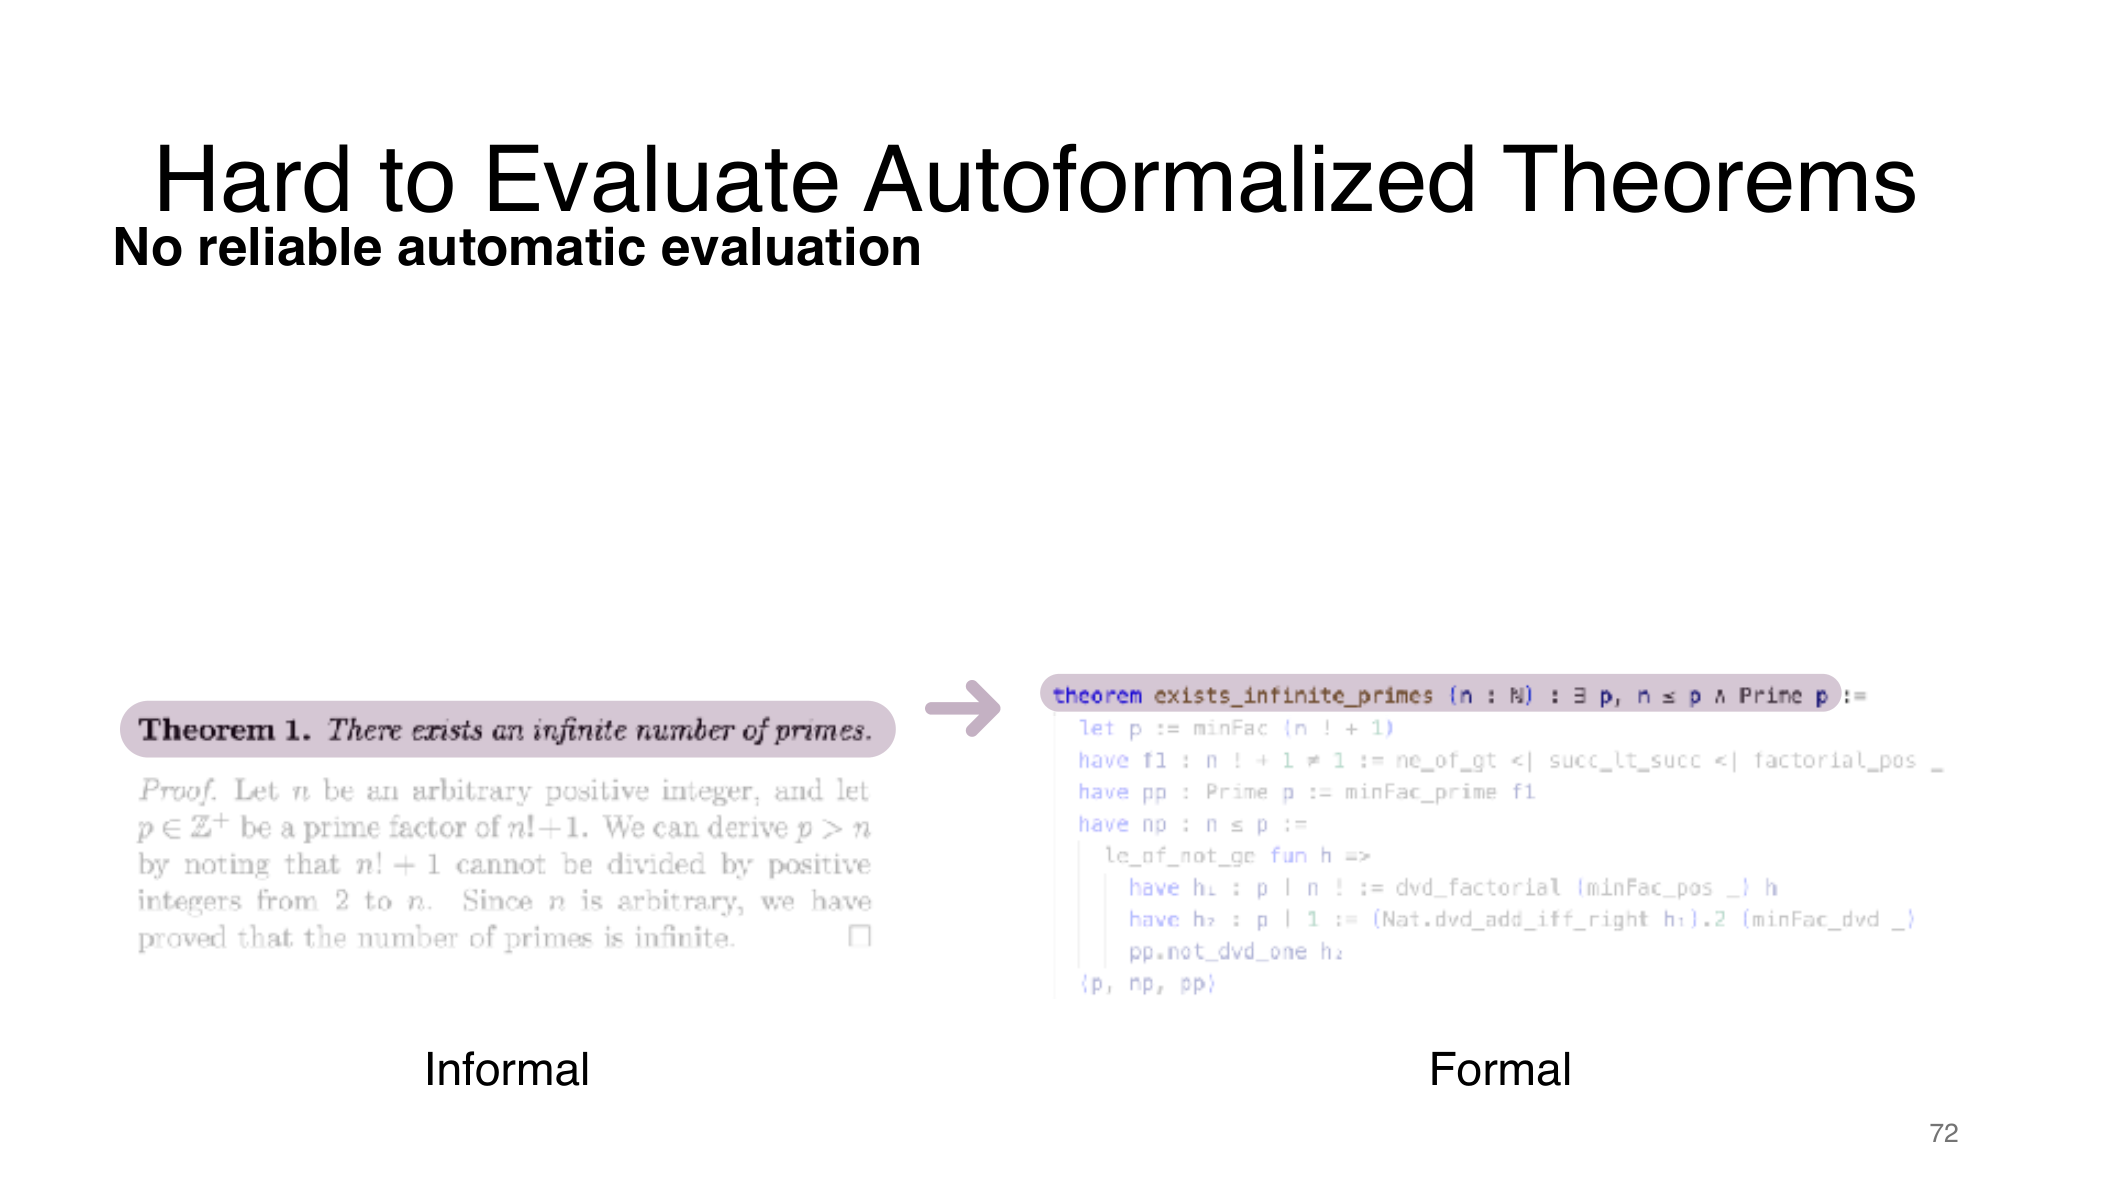
\includegraphics[width=0.80\textwidth]{figures/lec09_fig_013.png}
\caption{Theorem-level evaluation 的难点。}
\end{figure}

autoformalized theorem 的评估难点，在于“表面形式不同但语义相同”的情况太多。一般情形下，很难自动判断一个 formal statement 是否真正等价于原始问题。等价性检查的理想形式是
\[
T_{1} \equiv T_{2} \iff \left(T_{1}\Rightarrow T_{2}\right)\wedge\left(T_{2}\Rightarrow T_{1}\right).
\]
但这要求我们已经能在目标形式系统里证明双向蕴含，本身就不容易。因此 BLEU 之类表面指标没用，纯人工评估又昂贵。

\subsection{reasoning gaps：proof autoformalization 比 theorem autoformalization 更难}

\begin{figure}[H]
\centering
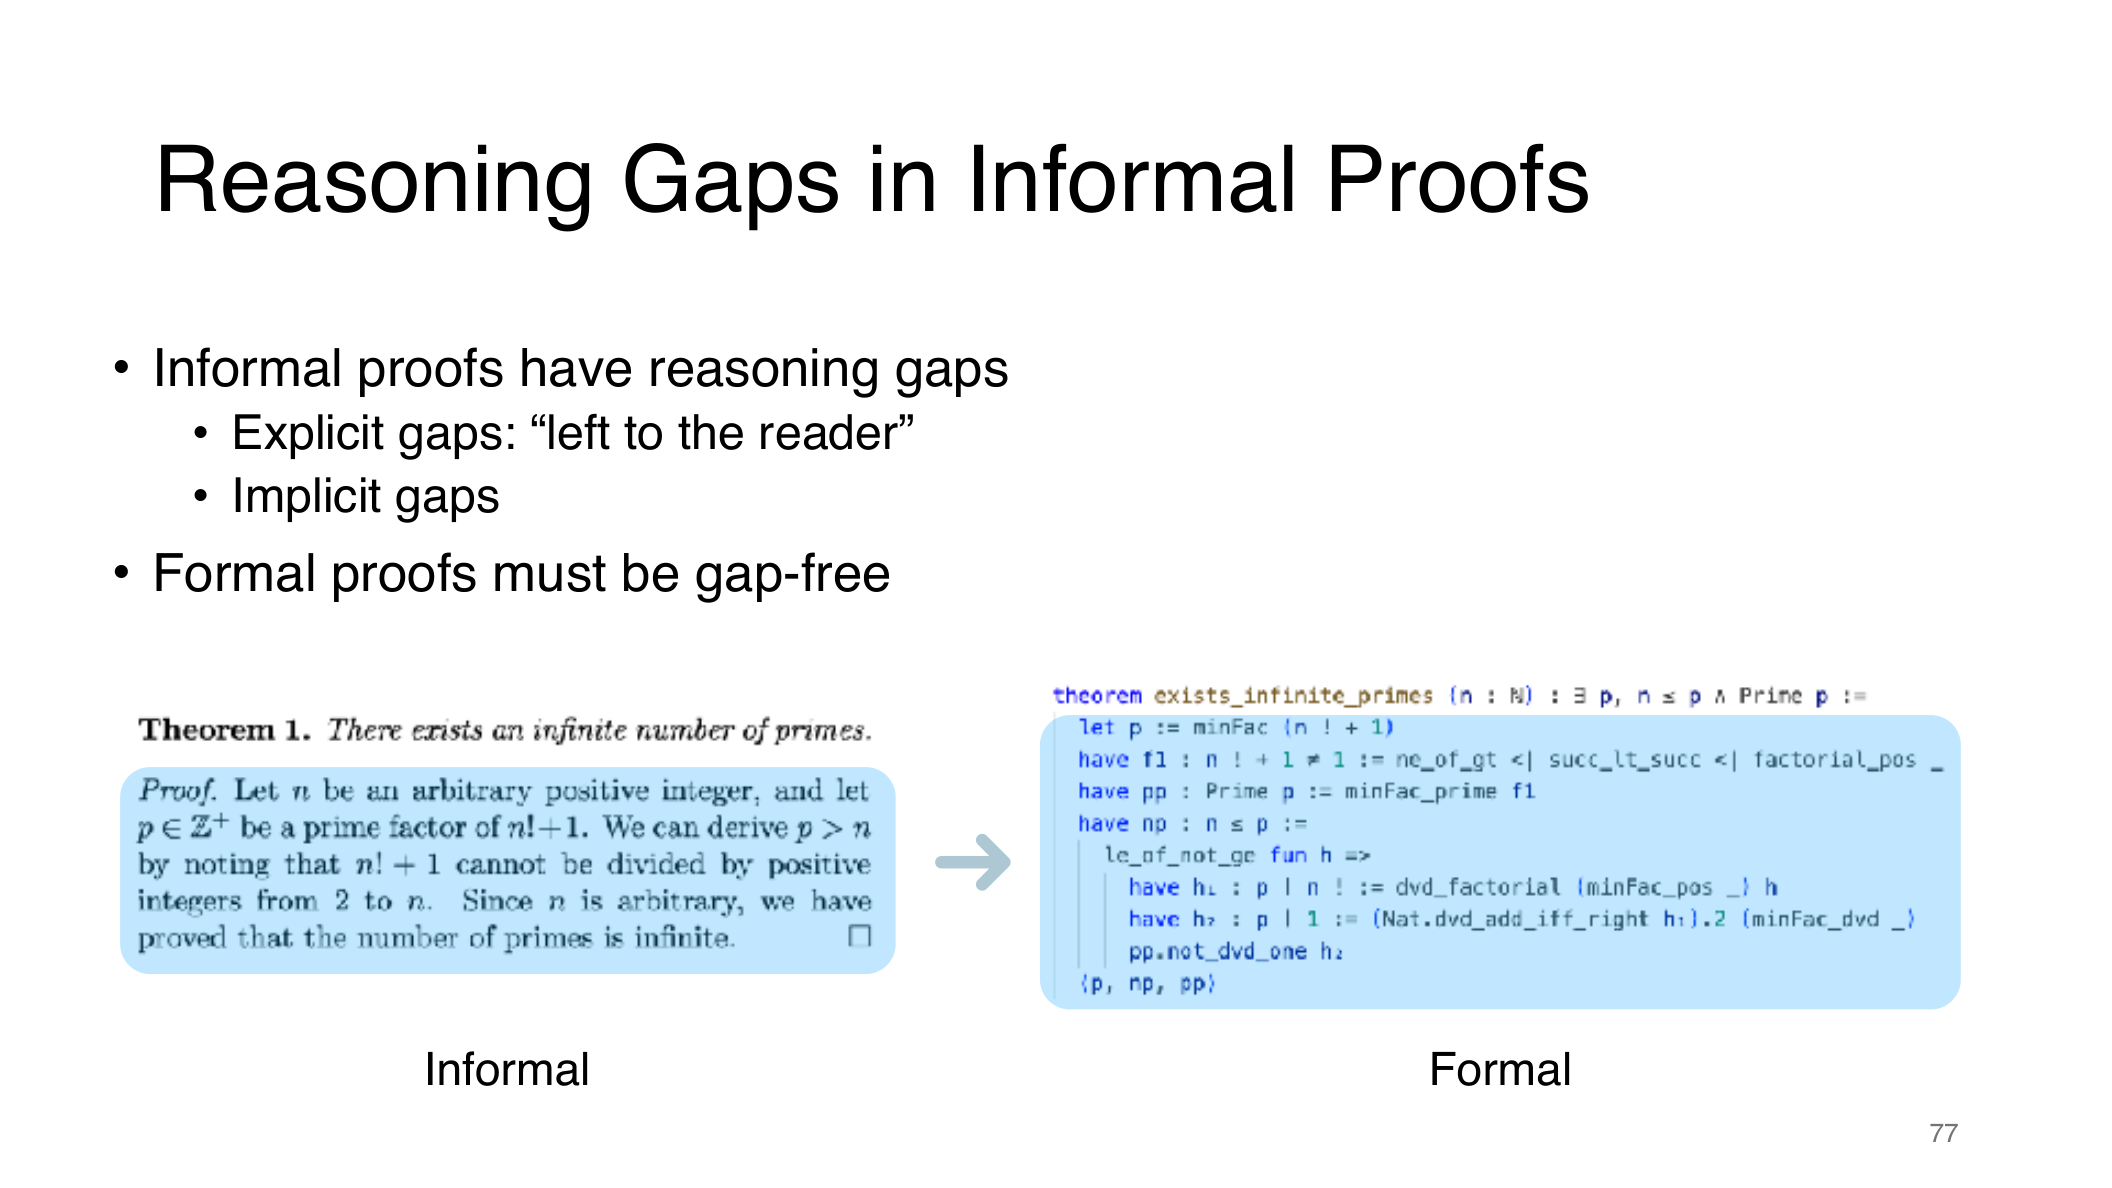
\includegraphics[width=0.80\textwidth]{figures/lec09_fig_014.png}
\caption{Informal proofs 普遍存在 reasoning gaps。}
\end{figure}

自然语言证明经常说“剩余步骤类似”“易证”“由图可见”。人类读者会自动补齐，但 formal proof 不能容忍这些跳步。因此 proof autoformalization 的难点不是把句子翻译成另一种语法，而是要\textbf{恢复作者默认省略的推理。} 这一步有时甚至需要重新发明中间 lemma，而不只是抄写。

\begin{lstlisting}
informal theorem or proof text
-> language model proposes a formal theorem statement
-> optional equivalence / semantic checking
-> theorem prover fills missing proof steps or rejects the candidate
\end{lstlisting}

\subsection{Euclidean geometry：diagrammatic reasoning 为什么特别难}

\begin{figure}[H]
\centering
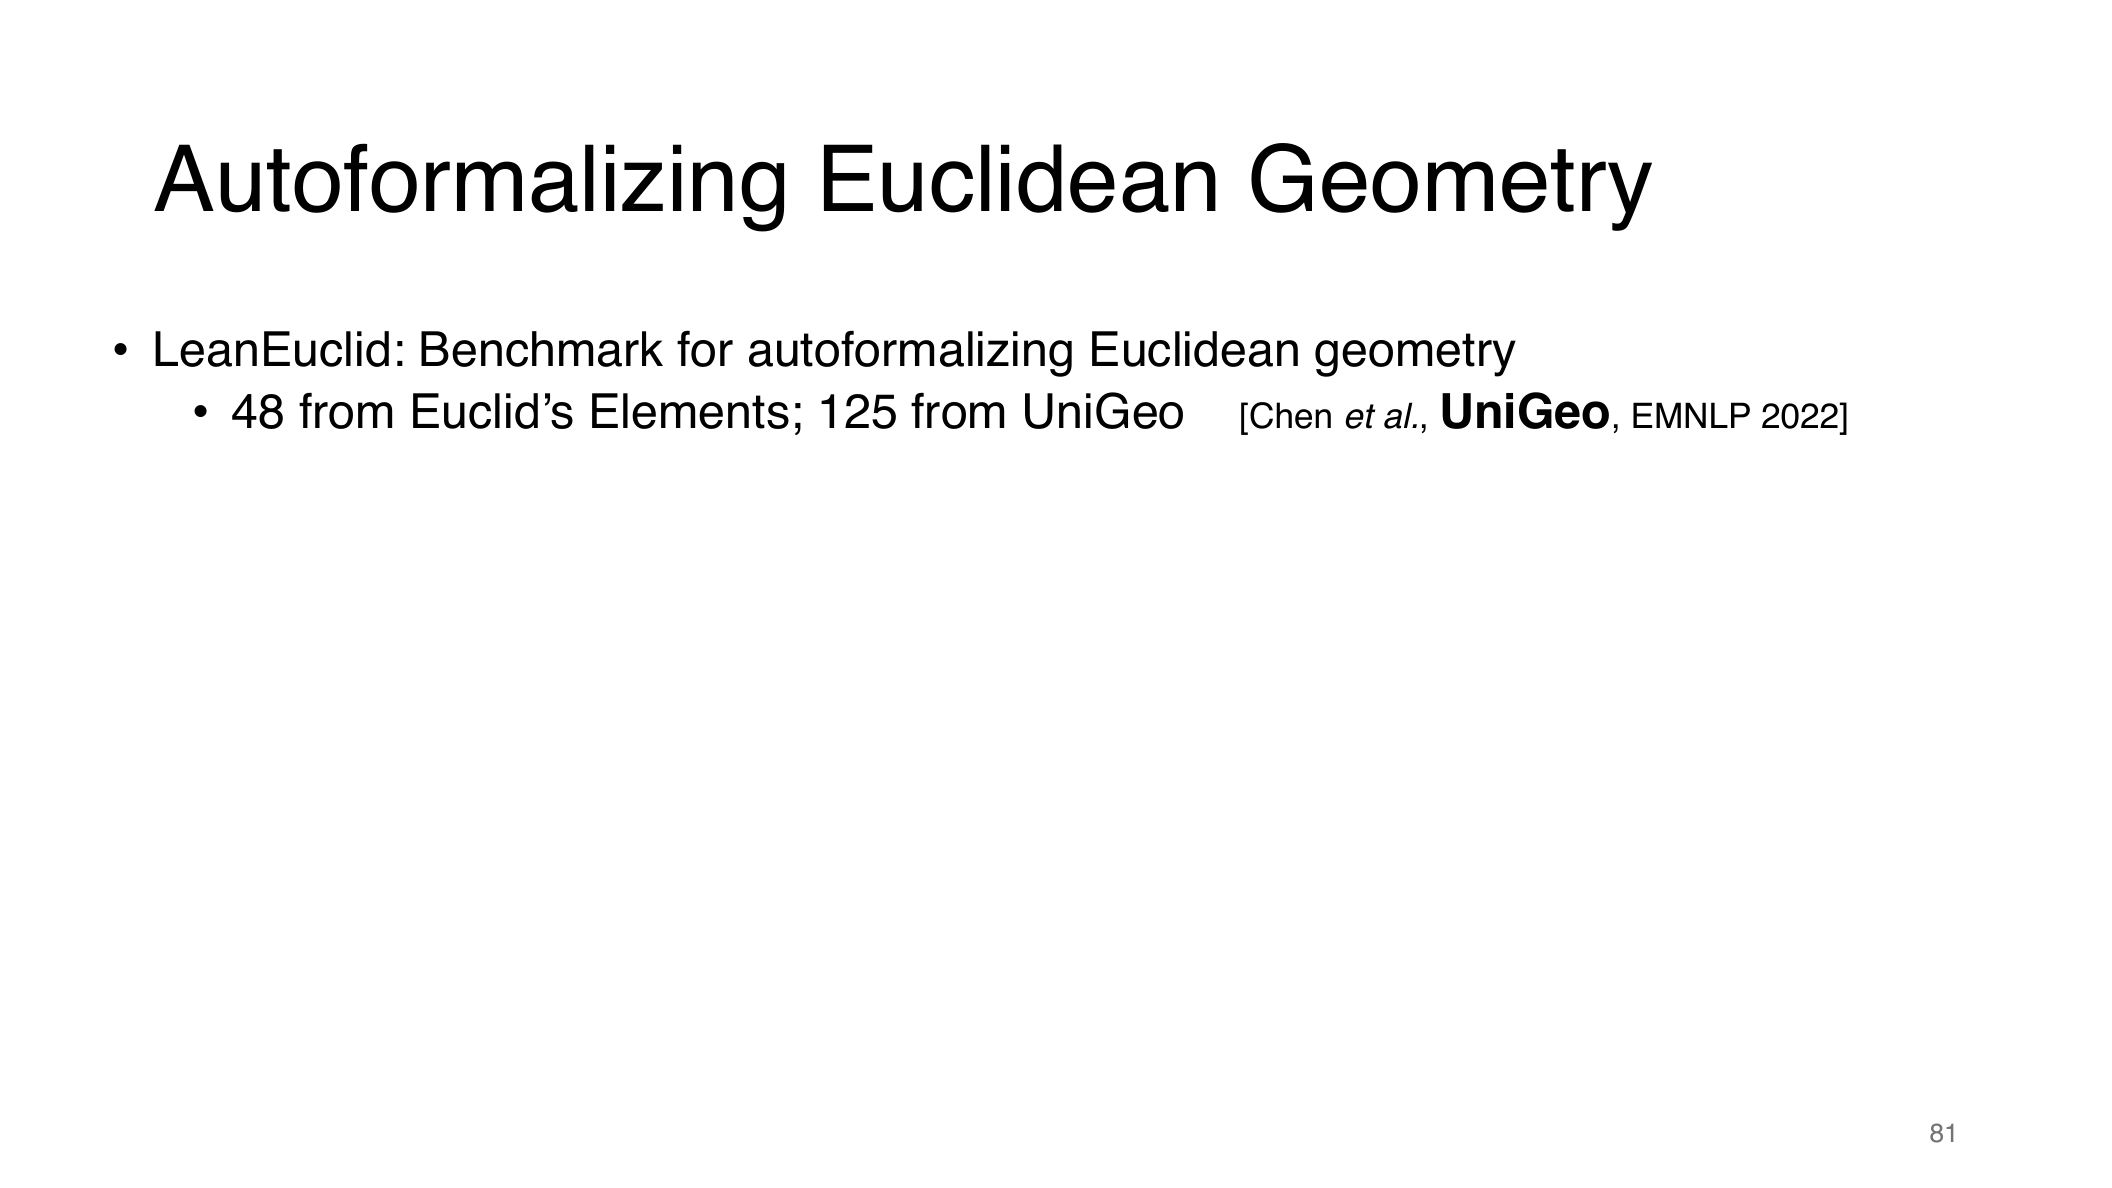
\includegraphics[width=0.80\textwidth]{figures/lec09_fig_015.png}
\caption{LeanEuclid：geometry autoformalization benchmark。}
\end{figure}

\begin{figure}[H]
\centering
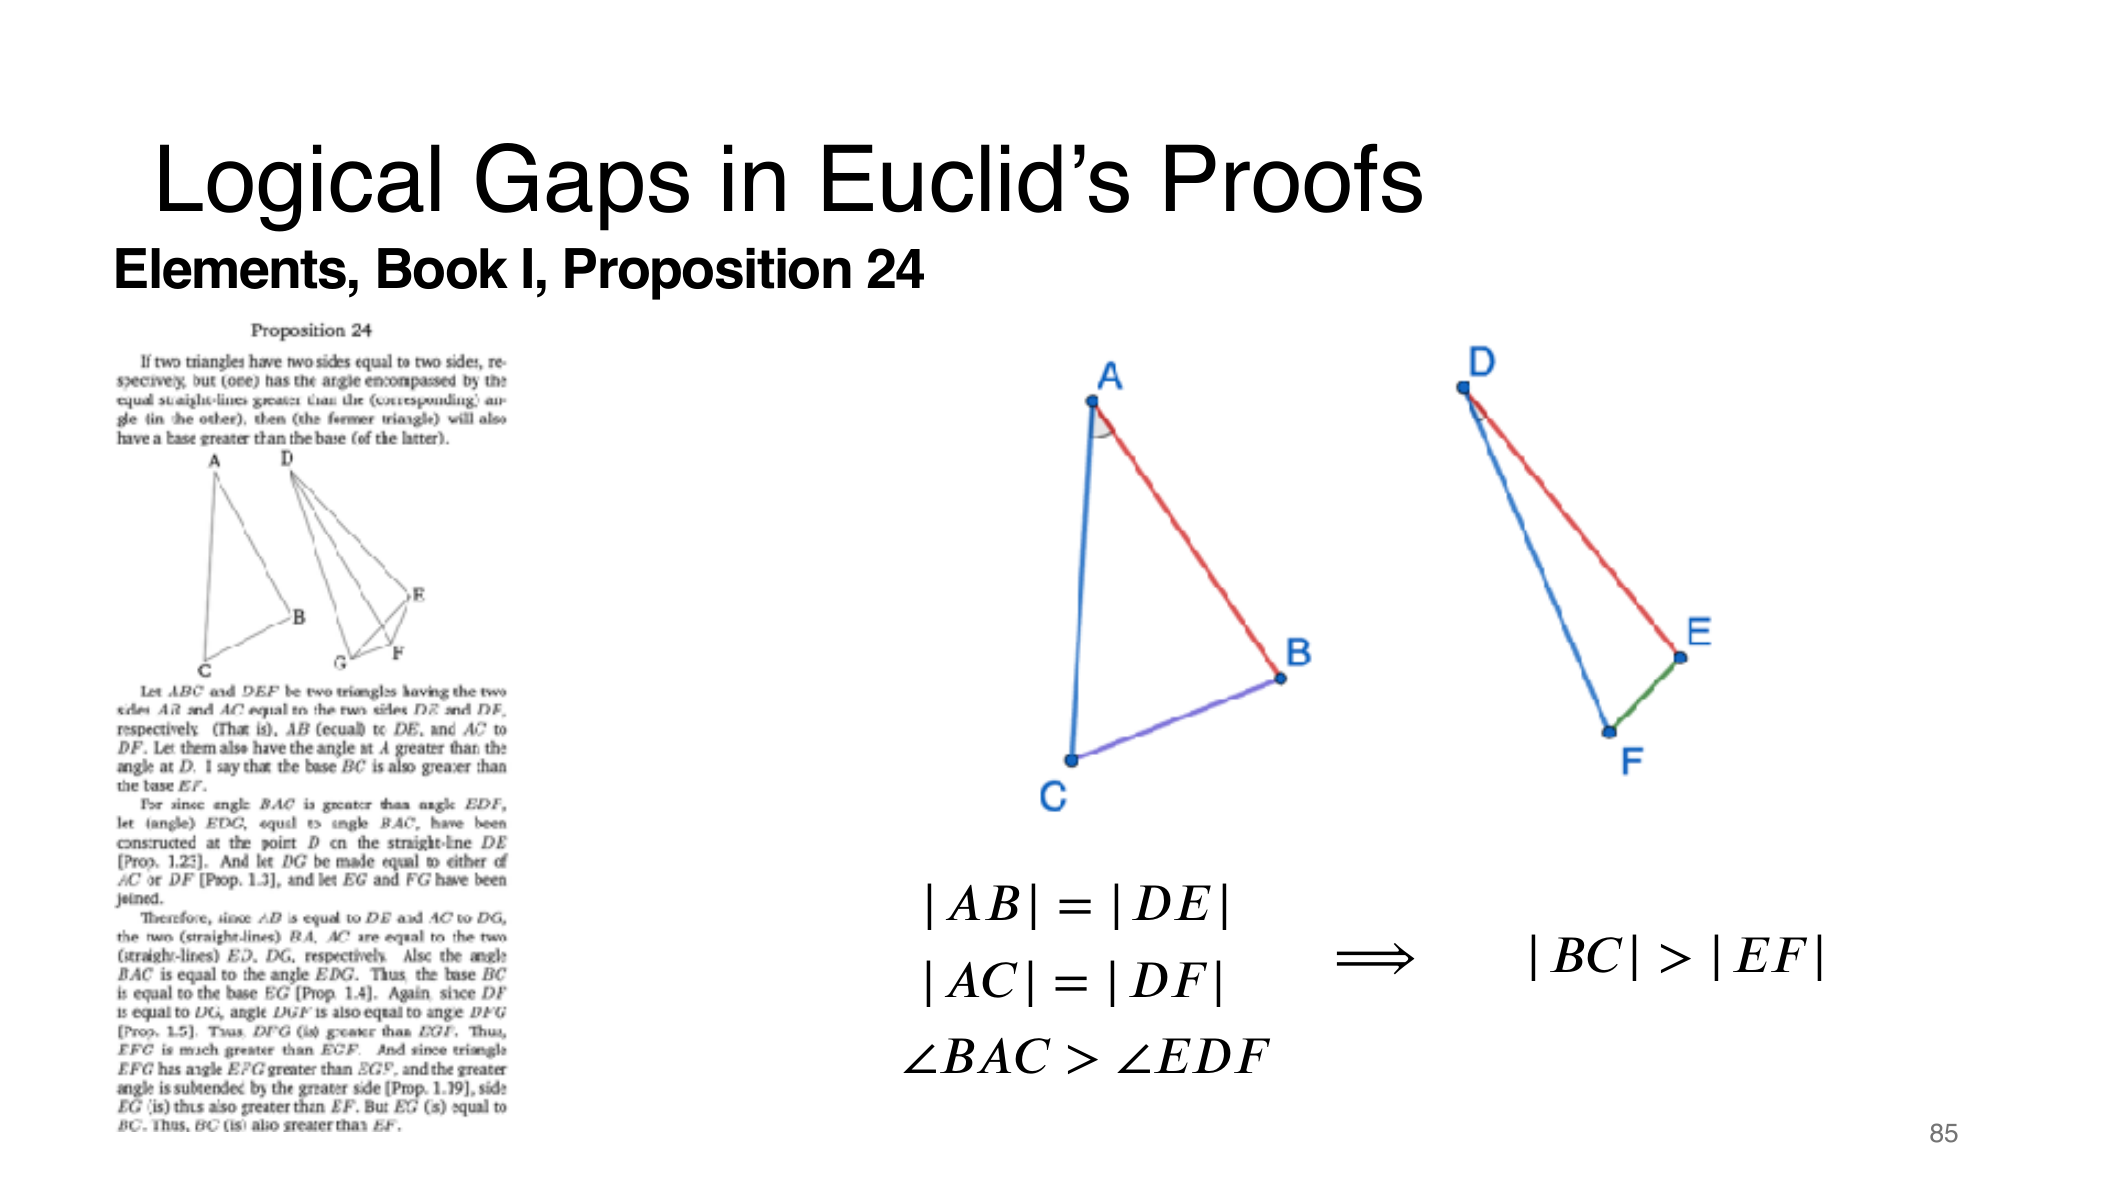
\includegraphics[width=0.80\textwidth]{figures/lec09_fig_016.png}
\caption{Euclid proofs 中的 logical gaps。}
\end{figure}

几何证明之所以难，不只因为定理本身复杂，而是因为很多推理建立在图形直觉上。例如“这两条线显然相交在某处”“该三角形显然是等腰”，在人类眼里依赖图即可成立，但 formal system 需要把所有这些条件显式写出来。

这也是《Autoformalizing Euclidean Geometry》那篇 reading 的关键洞见：要想让 LLM 负责 autoformalization，必须先把 diagrammatic information 通过 theorem provers、SMT solvers 或专门 formal system 提取出来，否则语言模型面对的是一个语义残缺的输入。

\subsection{equivalence checking 与 diagrammatic formal system}

\begin{figure}[H]
\centering
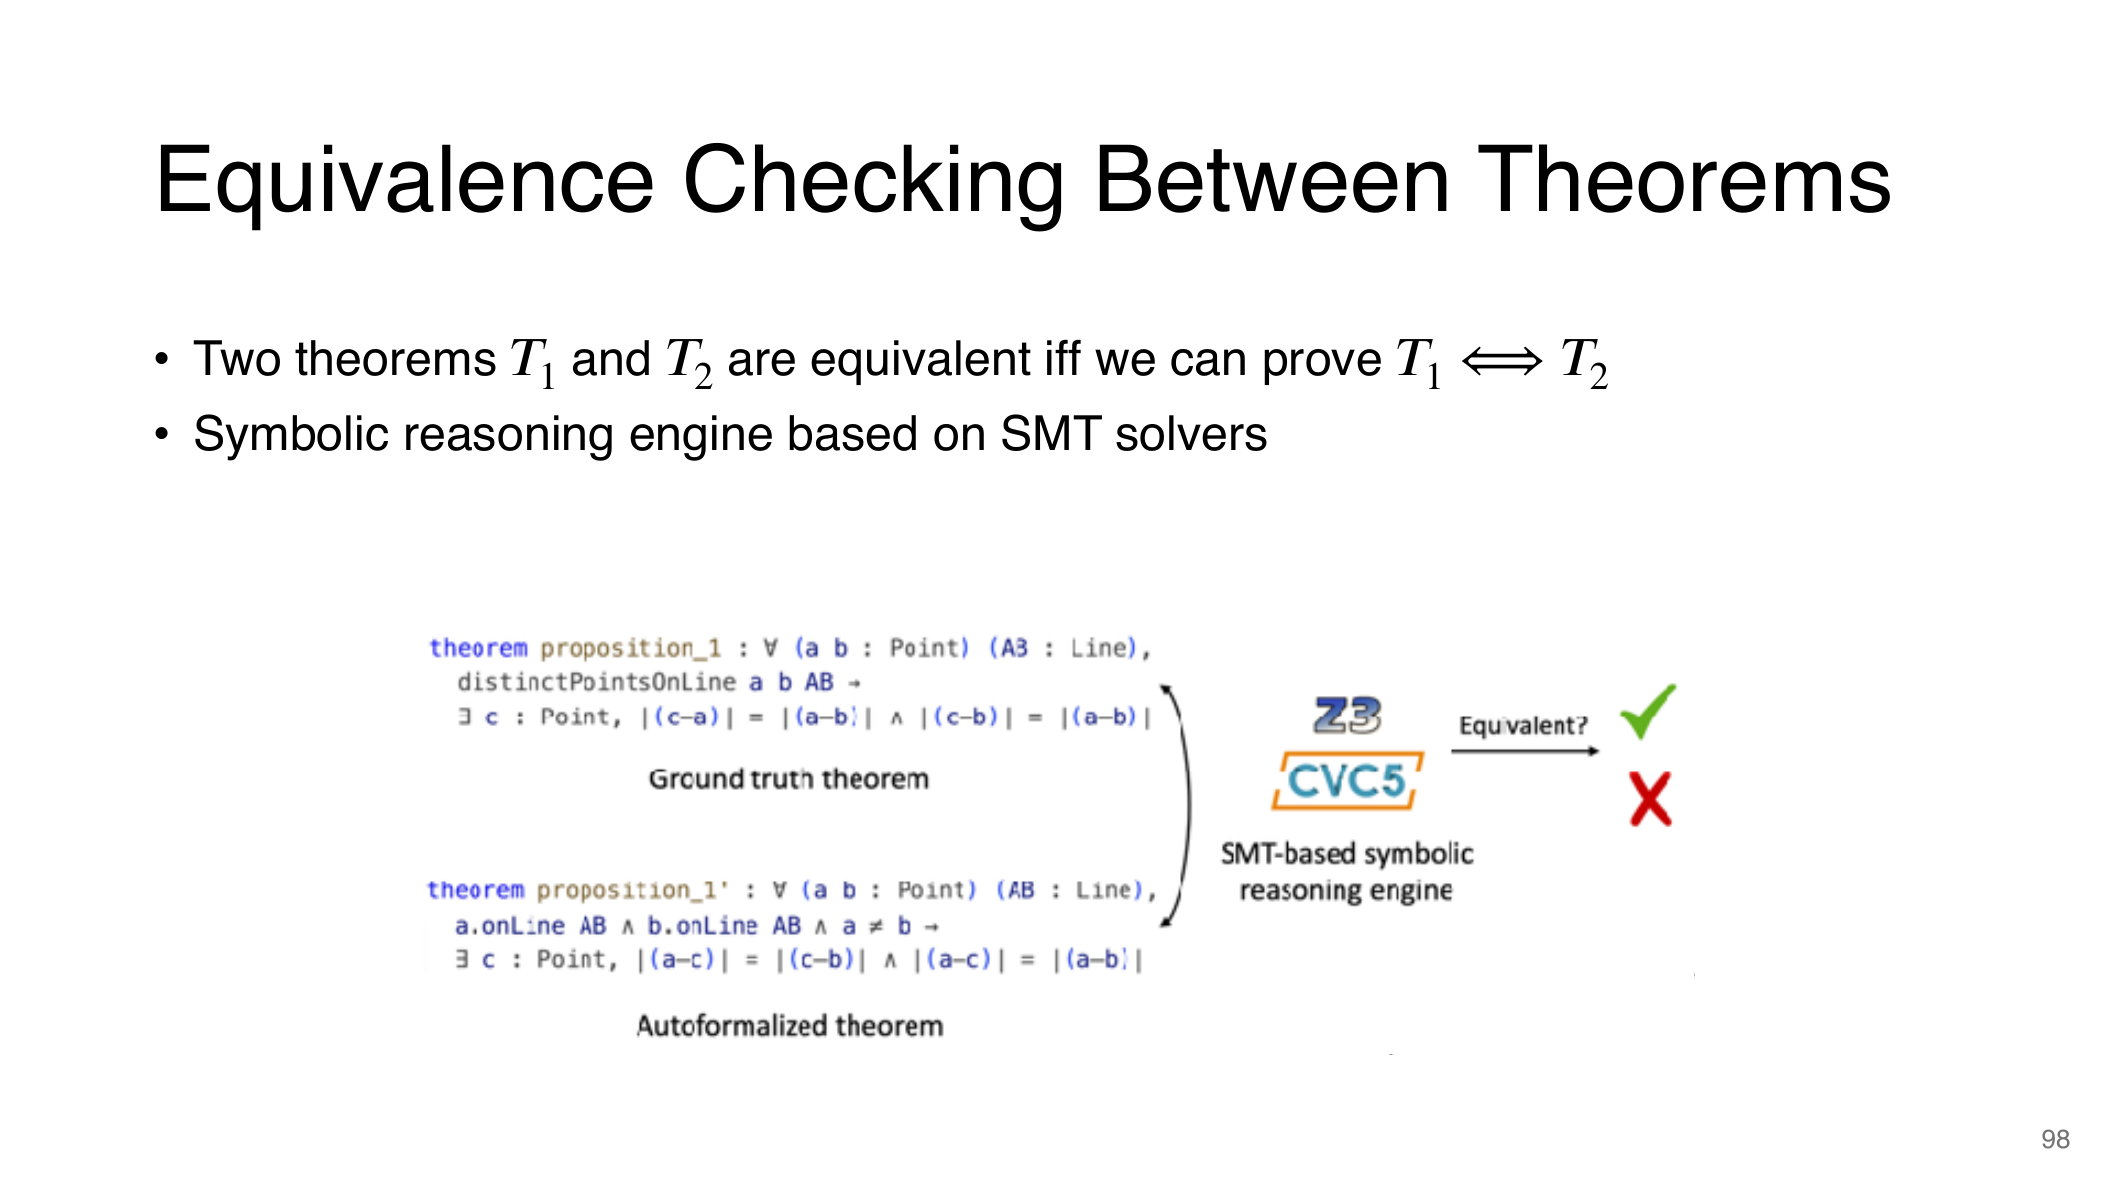
\includegraphics[width=0.78\textwidth]{figures/lec09_fig_017.png}
\caption{Theorem equivalence checking 的理想形式。}
\end{figure}

\begin{figure}[H]
\centering
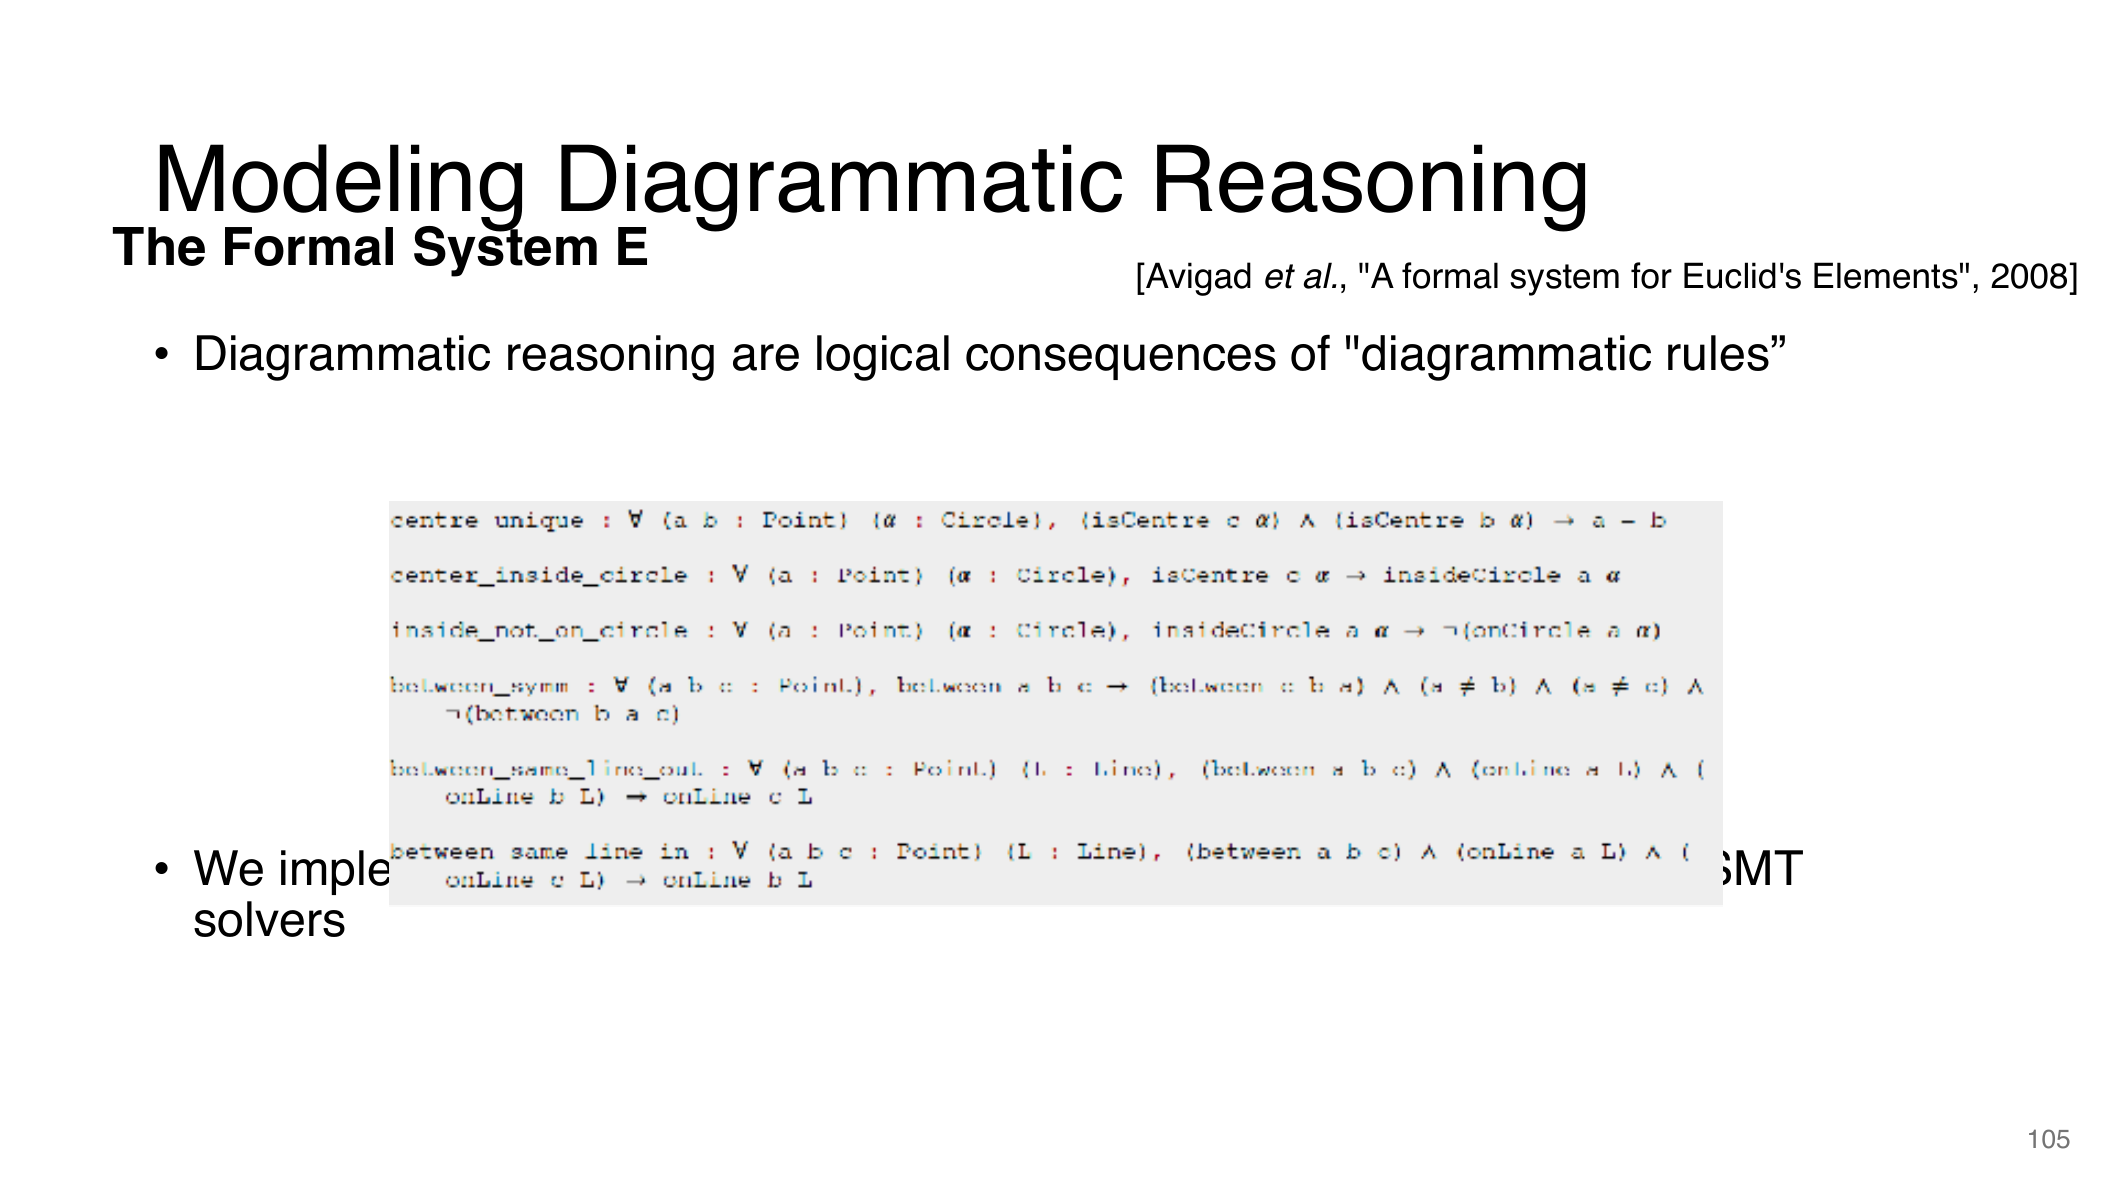
\includegraphics[width=0.78\textwidth]{figures/lec09_fig_018.png}
\caption{把 diagrammatic reasoning 写进 formal system。}
\end{figure}

Lecture 最后给出的方向不是“再堆更大的 LLM”，而是：针对特定 domain，把原本隐式的 reasoning 规则写进 formal system。例如 geometry 中的图示规则，如果能被建模成 formal rule，那么 autoformalization 和 theorem proving 都会得到更可靠的结构支撑。

\section{关键论文与课程 readings 的连接}

\subsection{LeanDojo：开放环境的重要性}

LeanDojo 对本讲的意义，不只是一个具体模型分数，而是它把 theorem proving 的基础设施、数据和 evaluation 标准化了。没有这样的环境，后续所有 retrieval、search 和 agent-harness 设计都会变得脆弱且不可复现。

\subsection{Autoformalization with Large Language Models：正式定义任务}

这篇论文把 autoformalization 作为独立任务立住。它告诉我们，系统必须先学会“把问题写对”，然后 theorem prover 才有机会“把证明找对”。这与 L08 中 manual formalization 仍不可或缺的现实形成直接呼应。

\subsection{Autoformalizing Euclidean Geometry：geometry 是试金石}

这篇论文的重要性在于，它把 geometry 中的 diagrammatic reasoning 变成可研究对象。它说明 autoformalization 的核心难点不是通用语法翻译，而是恢复隐含前提、处理图示信息并构造可验证的 formal semantics。

\section{例子、反例、失败模式和边界条件}

\subsection{formal reasoning 的典型失败模式}

\begin{itemize}
\item \textbf{statement mismatch}：formal theorem 写错，后续 proving 再强也没有意义。
\item \textbf{premise overload}：premise 数量过大，retrieval 失败会让 prover 在错误知识子集上搜索。
\item \textbf{action explosion}：proof search 分支过多，局部采样无法稳定前进。
\item \textbf{semantic evaluation gap}：即使 checker 接受某个 theorem，也未必说明它忠实表达了原始问题。
\item \textbf{diagrammatic omission}：几何中的图形约束若未显式补齐，autoformalization 会系统性缺信息。
\end{itemize}

\subsection{与 verification 的边界}

verification 的作用是判断一个 formal object 是否成立；它不负责生成 theorem statement，不负责选择 premises，也不负责决定 search policy。因此“有 verifier”不等于“formal reasoning 问题已经解决”。这和安全章节里常见的一个教训类似：\textbf{checker 能发现部分错误，但不能替代建模与搜索本身。}

\section{与前后讲的联系}

L08 展示的是 formal mathematics 作为环境的吸引力；L09 则把这个环境内部的任务进一步拆开，说明其中哪些部分是 RL/search 问题，哪些是表示和语义问题。再往后看，这种“环境 + 表示 + 搜索 + 验证”的拆法，也会在安全 agent、coding agent 和 abstraction/discovery 章节中反复出现。

\section{本章小结}

本讲最大的贡献，是把“数学推理”从一个模糊标签拆成了多层任务：formal specification、verification、theorem proving、proof search、autoformalization。它同时给出三个关键结论：第一，proof assistant 提供了极其重要的环境反馈；第二，retrieval 与 domain structure 对 theorem proving 仍然关键；第三，autoformalization 的最大难点在于 informal proofs 中无处不在的语义缺口与图形推理。

\section{复习题}

\begin{enumerate}
\item 为什么当前 math LLM 的 recipe 不能自动解决 formal reasoning？
\item formal specification 和 theorem proving 的输入输出分别是什么？
\item ReProver 中 retrieval 的作用是什么？
\item theorem equivalence checking 为什么困难？
\item geometry autoformalization 为什么比普通符号翻译更难？
\end{enumerate}

\section{深入思考题}

\begin{enumerate}
\item 如果 verification 完美，但 theorem statement 经常写错，系统会在什么环节失真？
\item theorem proving 是否更像 coding agent、web agent，还是更像 game-playing agent？为什么？
\item 针对特定数学子域引入专门 formal system，是否会破坏通用性？应如何权衡？
\end{enumerate}

\section{延伸阅读}

\begin{itemize}
\item \emph{LeanDojo: Theorem Proving with Retrieval-Augmented Language Models}
\item \emph{Autoformalization with Large Language Models}
\item \emph{Autoformalizing Euclidean Geometry}
\item Formal Mathematical Reasoning position paper
\end{itemize}

\end{document}
